\documentclass[aspectratio=169]{beamer}

\usepackage{amsmath, amssymb, amsxtra, amsthm, amsfonts}
\usetheme{moloch}
\usecolortheme{beaver}
\setbeamertemplate{footline}
{
  \leavevmode%
  \hbox{%
    \begin{beamercolorbox}[wd=.5\paperwidth,ht=2.25ex,dp=1ex,center]{author in head/foot}%
      \usebeamerfont{author in head/foot}\insertsection
    \end{beamercolorbox}%
    \begin{beamercolorbox}[wd=.5\paperwidth,ht=2.25ex,dp=1ex,right]{date in head/foot}%
      \usebeamerfont{date in head/foot}\inserttitle\hspace*{2em}
      \insertframenumber{} / \inserttotalframenumber\hspace*{2ex}
    \end{beamercolorbox}}%
  \vskip0pt%
}
\makeatother

\usepackage[english]{babel}
\usefonttheme{serif}

\usepackage{mathtools}
\usepackage{graphicx}
\usepackage{bm}
\usepackage{color}
\usepackage[dvipsnames,table]{xcolor}
\usepackage{tikz}
\usepackage{stanli}
\usepackage{verbatim}
\usepackage{tikz}
\usetikzlibrary{shapes,calc,through,3d,patterns}
\usetikzlibrary{decorations.pathreplacing}
\usetikzlibrary{arrows.meta,calc,positioning}

\usepackage{pgfplots}
\usepackage{siunitx} % For formatting numbers
\usepackage{hyperref}
\hypersetup{colorlinks=true,linkcolor=darkred}
\usepackage{multicol}
\usepackage[absolute,overlay,]{textpos}
\usepackage{pgfplots}
\pgfplotsset{width=10cm,compat=1.9}
\usepackage{subcaption}
\usepackage{multirow}
\usepackage{bbding}
\usepackage{arydshln}
\usepackage{mathtools}
\usepackage{tcolorbox}
\usepackage{animate}

\textblockorigin{80mm}{45mm}


\newtheorem{thm}{Theorem}
\newtheorem{cor}[thm]{Corollary}
\newtheorem{prop}[thm]{Proposition}
\newtheorem{lem}[thm]{Lemma}
\theoremstyle{remark}
\newtheorem*{rem}{Remark}

%Block def
\definecolor{darkred}{rgb}{0.6,0,0}
\setbeamertemplate{blocks}[rounded][shadow=false]
\setbeamercolor{block title}{bg=darkred!15,fg=black}
\setbeamercolor{block body}{bg=darkred!5,fg=black}

\setbeamercolor{itemize item}{fg=darkred}
\setbeamercolor{itemize subitem}{fg=darkred}
\setbeamercolor{itemize subsubitem}{fg=darkred}
\setbeamercolor{enumerate item}{fg=darkred}
\setbeamercolor{button}{bg=gray!30,fg=darkred}

\setbeamertemplate{itemize item}[square]
\setbeamertemplate{itemize subitem}[circle]
\setbeamertemplate{itemize subsubitem}[triangle]
\setbeamertemplate{enumerate items}[circle]
\setbeamercolor{item projected}{bg=darkred}

\newcommand{\bolddelta}{\boldsymbol\delta}
\newcommand{\boldxi}{\boldsymbol\xi}
\DeclareMathOperator*{\A}{\text{\raisebox{-0.2cm}{\Huge A}}}




\title{Dynamic analysis of Reissner-Mindlin plates}
\subtitle{Special structural elements}
\author{ME473 Dynamic finite element analysis of structures}
\institute{Stefano Burzio}
\date{2025}

\begin{document}
\usenavigationsymbolstemplate{}
{\setbeamertemplate{footline}{}

  \frame{\titlepage
    \begin{tikzpicture}[overlay, remember picture]
      \node[anchor=north east, xshift=-.9cm] at (current page.north east) {
\includegraphics[width=2cm]{../images/epfl_logo.png}};
      \node[anchor=south east, xshift=-.87cm, yshift=.05cm] at (current page.south east)  {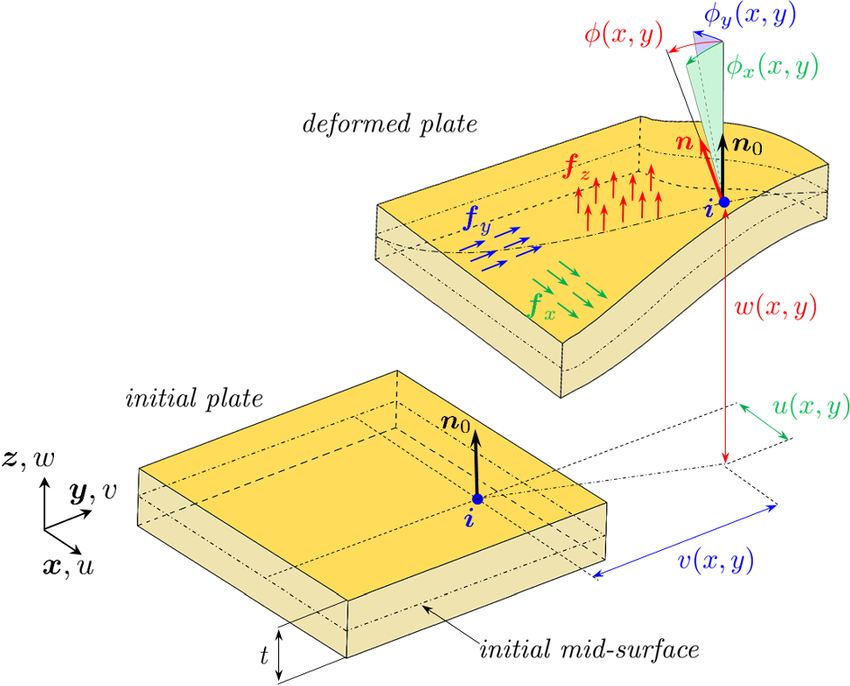
\includegraphics[height=4cm]{../images/ReissnerMindlin.png}};
    \end{tikzpicture}
  }

  \begin{frame}{Where do we stand?}
    \begin{center}
      \begin{tabular}{|c|l|l|l|}
        \hline
        \rowcolor{darkred!20}\textbf{Week} & \textbf{Module}                                & \textbf{Lecture topic}             & \textbf{Mini-projects} \\
        \hline

        1                                  & \multirow{5}{7em}{Linear elastodynamics}       & Strong and weak forms              &                        \\ \cline{1-1} \cline{3-4}
        2                                  &                                                & Galerkin method                    &                        \\ \cline{1-1} \cline{3-4}
        3                                  &                                                & Finite element method              & Groups formation       \\ \cline{1-1} \cline{3-4}
        4                                  &                                                & Systematization of the procedure   & Project 1 statement    \\
        \cline{1-1} \cline{3-4}
        5                                  &                                                & 3d elements, numerical integration &                        \\
        \hline
        6                                  & \multirow{5}{7em}{Special structural elements} & Bars and trusses                   &                        \\
        \cline{1-1} \cline{3-4} 7          &                                                & Planar beams                       & Project 1 submission   \\
        \cline{1-1} \cline{3-4} 8          &                                                & Frames and grids                   & Project 2 statement    \\

        \cline{1-1} \cline{3-4} 9          &                                                & Kirchhoff-Love plates              &                        \\
        \cline{1-1} \cline{3-4}
        10                                 &                                                & Reissner-Mindlin plates            &                        \\
        \hline
      \end{tabular}
    \end{center}
    \vspace{1cm}
  \end{frame}

  \begin{frame}
    \textbf{\large Summary}
    \begin{itemize}
      \item Recap week 9
      \item Reissner-Mindlin plate theory
      \item Thick plate bending elements
    \end{itemize}
    \vspace{.5cm}

    \textbf{\large Recommended readings}
    \begin{itemize}
      \item[(N)] Neto et al., Engineering Computation of Structures (chap. 6.2)
      \item[(P)] Petyt, Introduction to finite element vibration analysis (chap. 6)
      \item[(O)] Ochsner, PDE for classical structural members (chap. 7)
    \end{itemize}
  \end{frame}
}

\section{Recap week 9 \\ Vibrations of Kirchhoff-Love plates}
 {\setbeamercolor{background canvas}{bg=darkred!5}
  \setbeamercolor{block body}{bg=darkred!5,fg=black}

  \begin{frame}{Plate structure}
    \begin{itemize}
      \item Plate structures are geometrically similar to structures of the 2D plane stress problem, but it usually carries only \textbf{transversal loads} that lead to bending deformation of the plate.
      \item For example: floors of a building, aerospace and ships structures, etc...
    \end{itemize}
    \begin{center}
      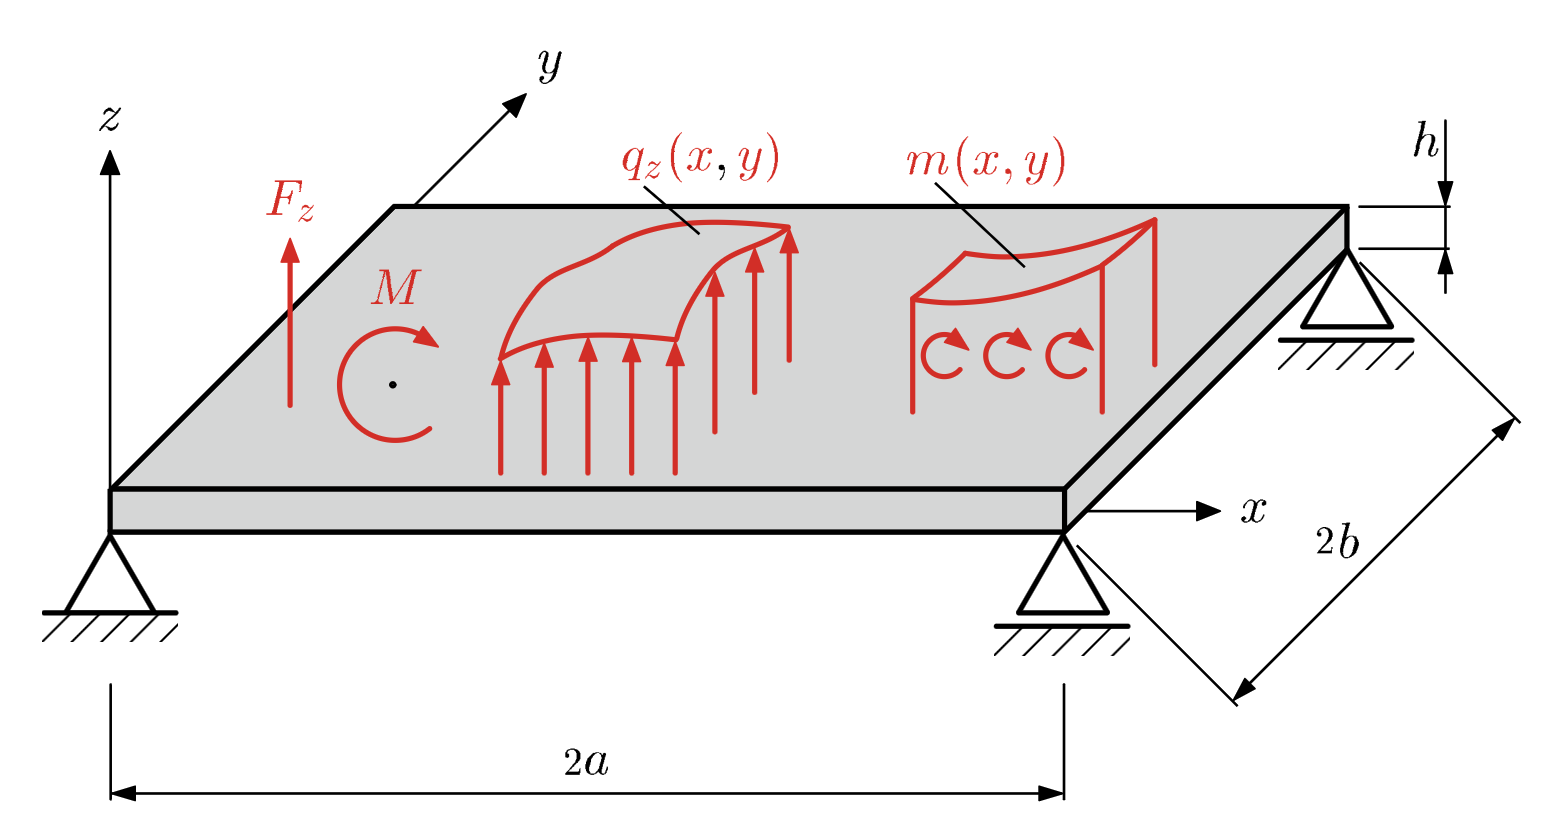
\includegraphics[width=8.5cm]{../images/Plate.png}
    \end{center}
    \emph{\footnotesize (Credit: (O))}
  \end{frame}

  \begin{frame}{Kirchhoff assumption}
    \textbf{Planarity and orthogonality of the cross-sectional planes} \\
    Bernoulli's hypothesis is valid, i.e. a cross-sectional plane stays plane and perpendicular to the middle surface in the deformed state.

    \begin{center}
      \begin{center}
        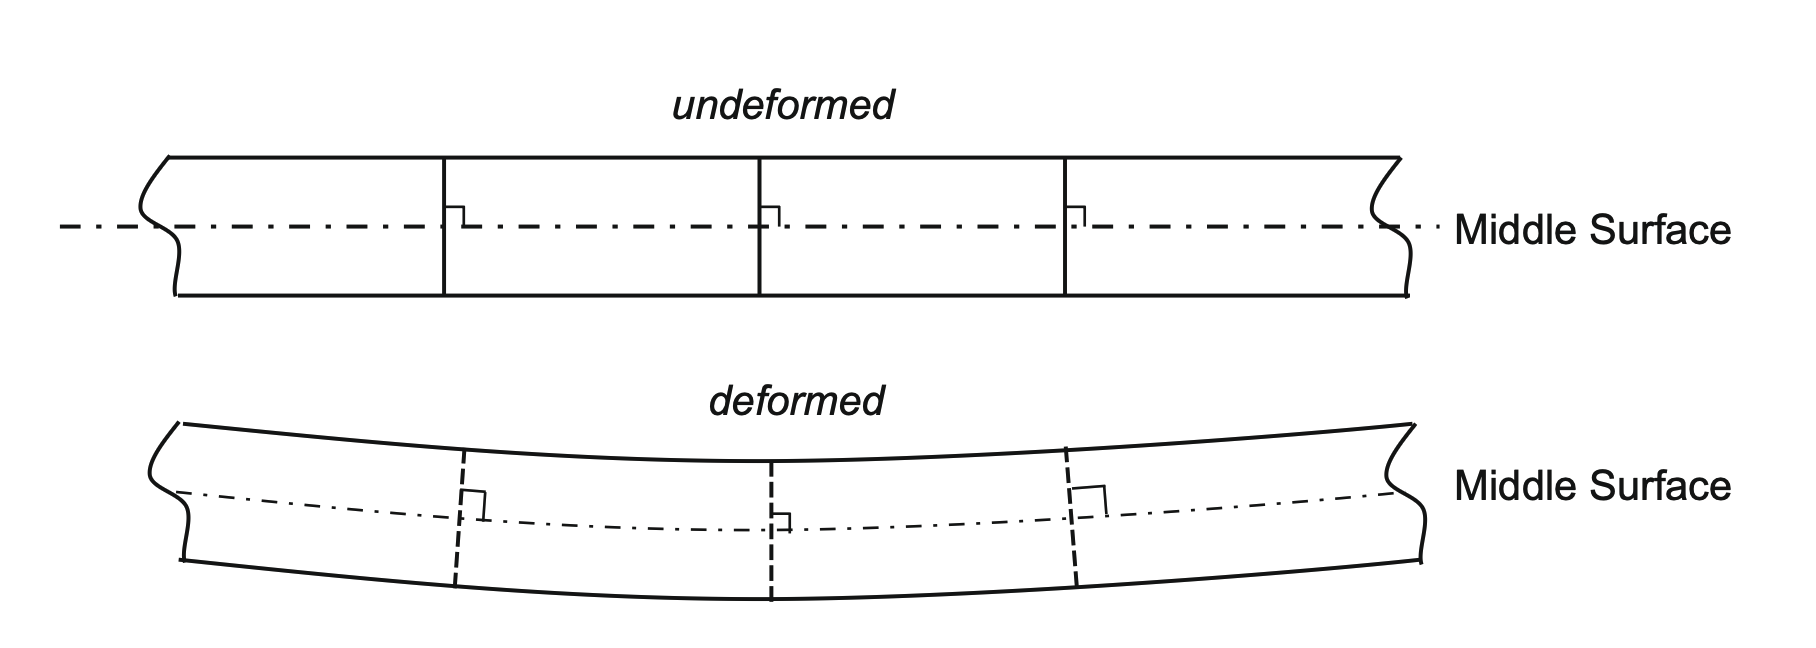
\includegraphics[width=6cm]{../images/KirchhoffPlateHp.png}
      \end{center}
    \end{center}
    \begin{tcolorbox}[colback=darkred!10,colframe=darkred!40!black]
      \begin{itemize}
        \item  Transverse shear strains are neglected $\varepsilon_{13}=\varepsilon_{23}=0$ due to the Bernoulli's hypothesis.
        \item Transverse normal strain is negligible $\varepsilon_{33} = 0$ due to the inextensibility of transverse fibers assumption.
      \end{itemize}
    \end{tcolorbox}
    \emph{\footnotesize (Credit: (N))}
  \end{frame}

  \begin{frame}{Finite element approximation of Kirchhoff-Love plate}
    \begin{itemize}
      \item Strong form
            $$
              \frac{h^3}{12}\boldsymbol{\nabla}_k^T \boldsymbol{C}\boldsymbol{\nabla}_ku_3+\rho h \ddot{u}_3=f_3 \qquad \text{  on  }\Omega\times]0,T[
            $$
      \item Weak form equation
            \[
              \frac{h^3}{12}\int_\Omega \, (\boldsymbol{\nabla}_k \delta u_3)^T\mathbf C \, \boldsymbol{\nabla}_k u_3  \, d\Omega + \int_\Omega \rho h\, \ddot u_3 \, \delta u_3 \, d\Omega = \int_\Omega f_3\, \delta u_3 \, d\Omega
            \]
      \item  Semi-discrete weak form
            $$\mathbf M\ddot{\mathbf q}(t)+\mathbf K\mathbf q(t)=\mathbf r(t)$$
    \end{itemize}

    \begin{tcolorbox}[colback=darkred!10,colframe=darkred!40!black]
      \begin{itemize}
        \item  \textbf{Adini-Melosh-Clough element (AMC)}: \\ 12 DOFs quadrangular, not conforming, thin plate bending element.
        \item  \textbf{Crouzeix–Raviart (CR)}: \\ 16 DOFs quadrangular, conforming, thin plate bending element.
      \end{itemize}
    \end{tcolorbox}
  \end{frame}

  \begin{frame}{Comparison: AMC vs CR plate bending element}

    \begin{columns}
      \begin{column}{0.5\textwidth}
        \begin{figure}[H]
          \begin{center}
            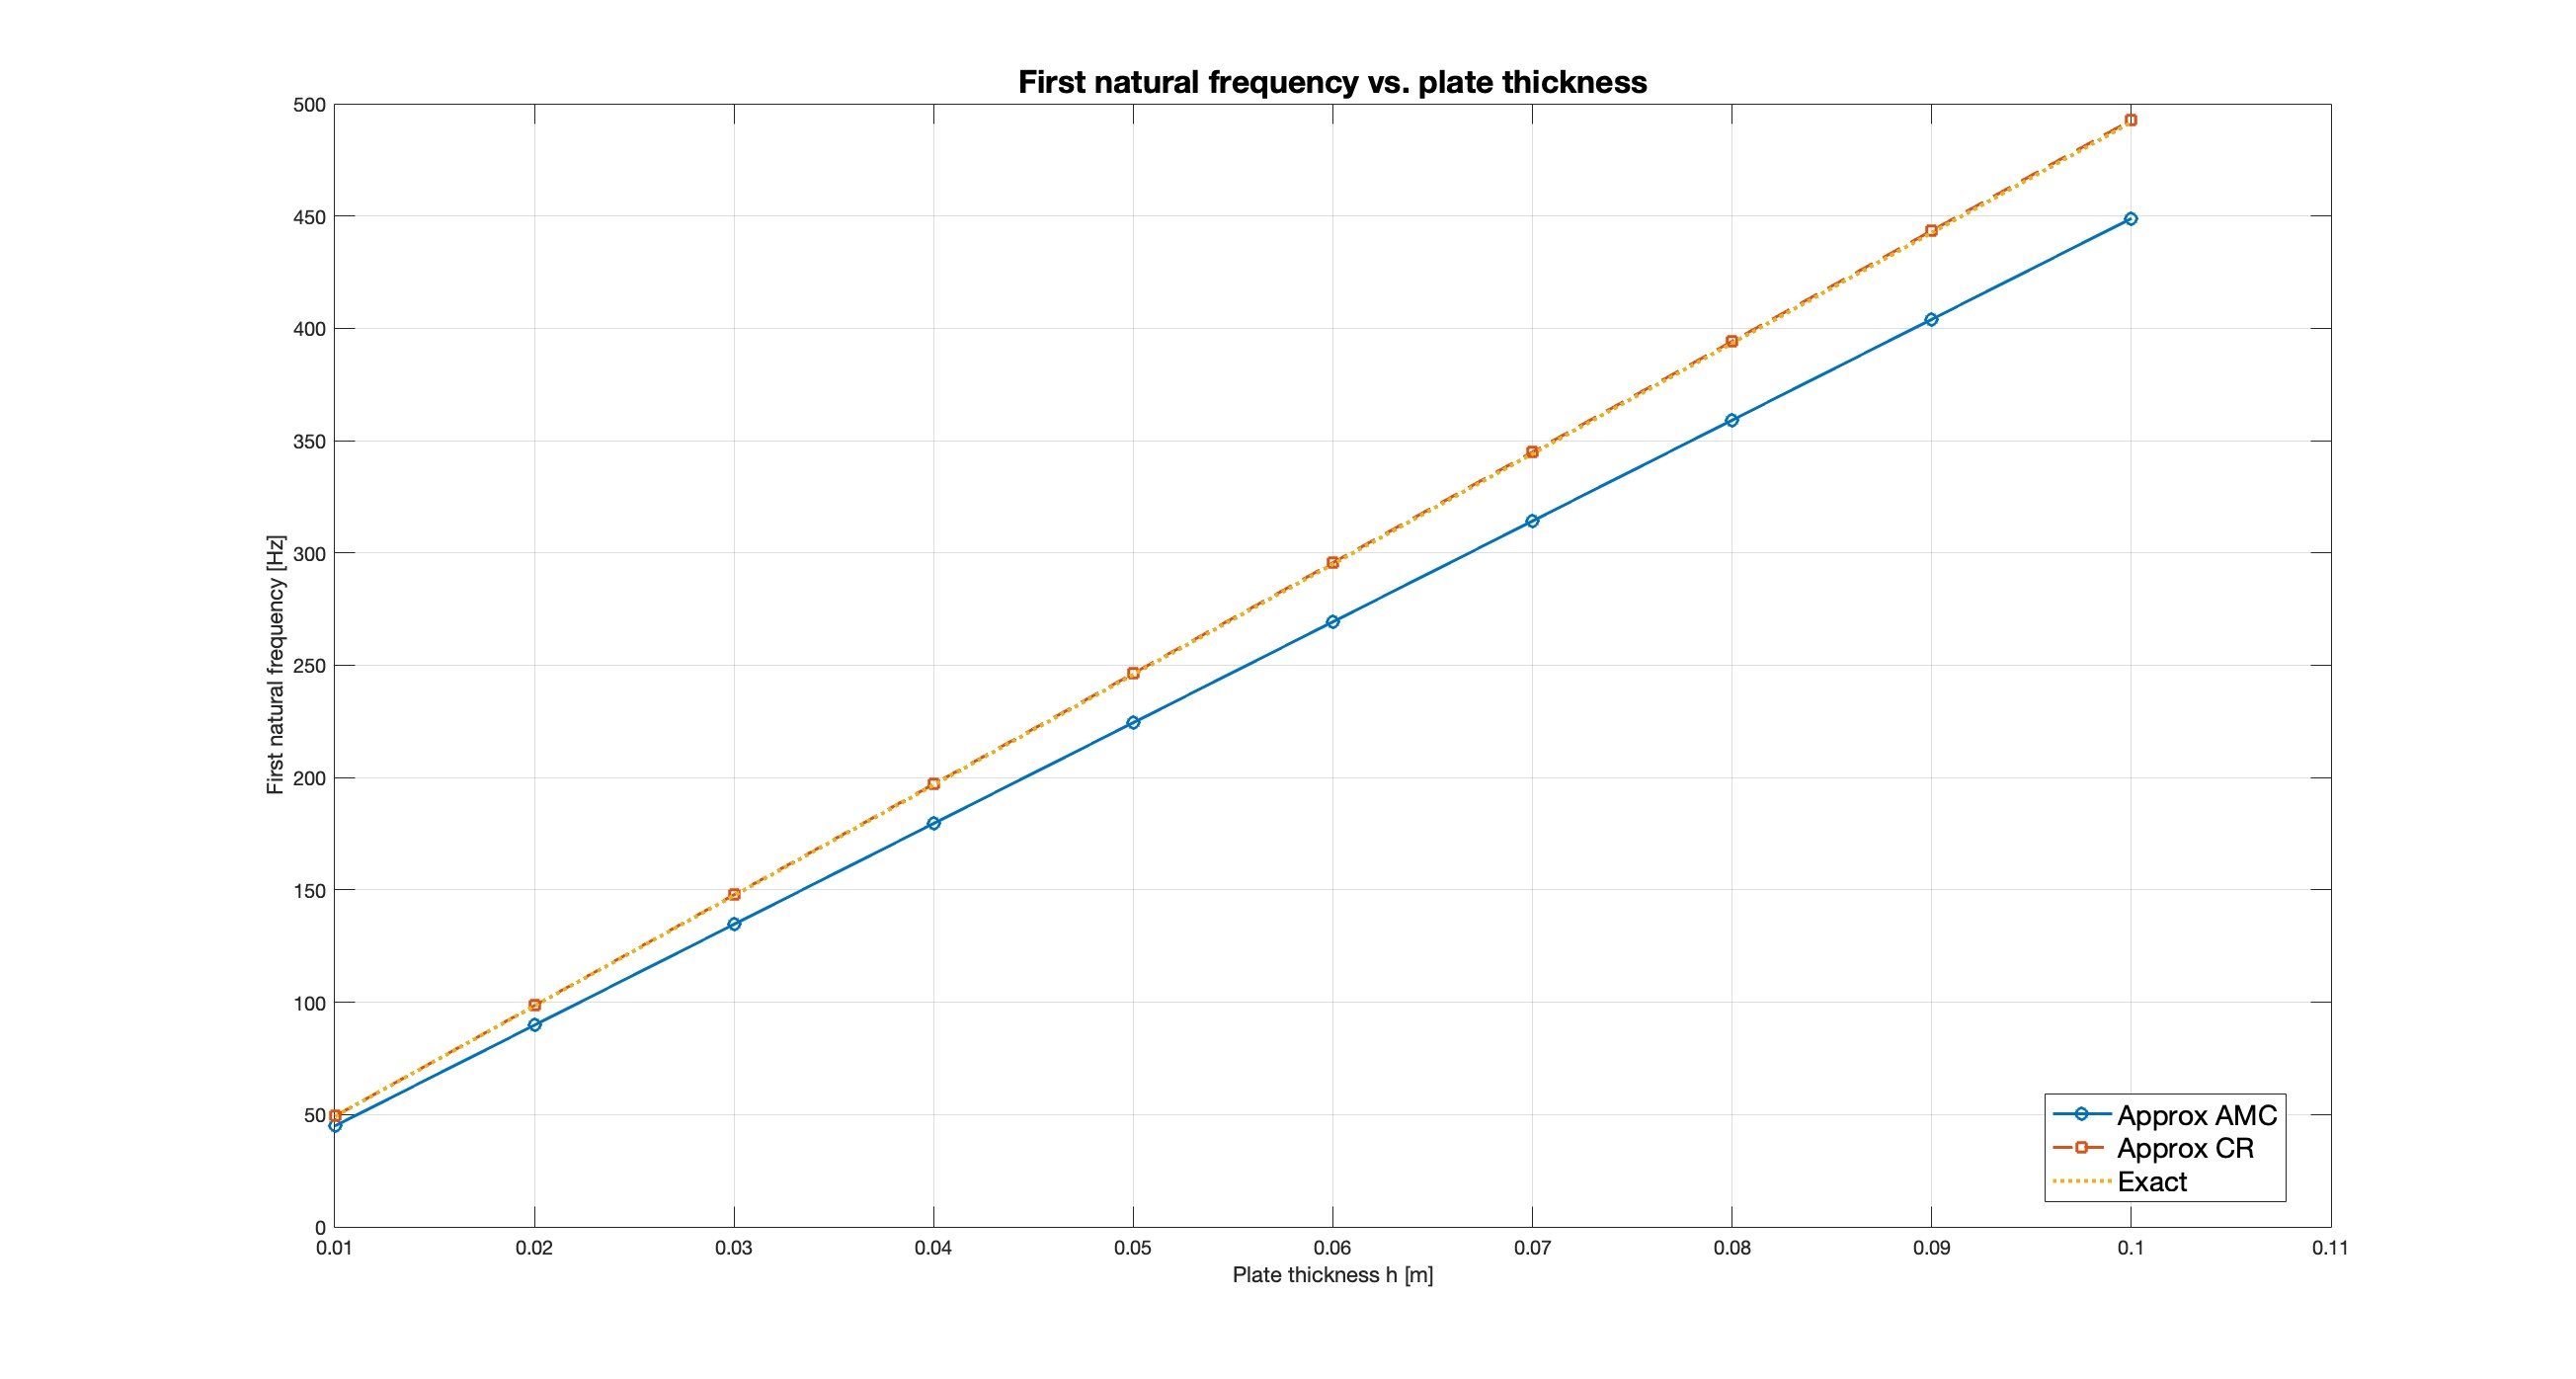
\includegraphics[height=4.8cm, width=7.5cm]{../images/CRandAMCThickness.jpg}
            \caption{Evolution of the approximated and exact fundamental frequencies with thickness for a SSSS square plate.}
          \end{center}
        \end{figure}      \end{column}
      \begin{column}{0.5\textwidth}
        \textbf{AMC element (\emph{Non conforming})}
        \begin{itemize}
          \item 3 degrees of freedom per node: \( u_3\), \( \theta_1 \), \( \theta_2 \).
          \item Only displacement \( u_3 \) is continuous across elements; rotations may have jumps.
        \end{itemize}
        \textbf{CR element (\emph{Conforming})}
        \begin{itemize}
          \item 4 degrees of freedom per node: \( u_3 \), \( \theta_1 \), \( \theta_2 \), and \(  \theta_{12} \).
          \item Displacement \( u_3 \) and rotations \( \theta_1, \theta_2 \) are continuous across element boundaries.
        \end{itemize}    \end{column}
    \end{columns}
  \end{frame}

  \begin{frame}{Selection of the displacement function}
    \vspace{-1cm}
    \begin{block}{}
      \textbf{Displacement approximation for AMC element}
      \begin{align*}
        {}^eu_3^h(x_1,x_2,t) = & \, {\color{darkred}a_1 + a_2 x_1 + a_3 x_2 + a_4 x_1^2 + a_5 x_1 x_2 + a_6 x_2^2} +                                              \\
        +                      & \,{\color{brown} a_7 x_1^3 + a_8 x_1^2 x_2 + a_9 x_1 x_2^2 + a_{10} x_2^3} + {\color{orange}a_{11} x_1^3 x_2 + a_{12} x_1 x_2^3}
      \end{align*}
    \end{block}

    \begin{block}{}
      \textbf{Displacement approximation for CR element}
      \begin{align*}
        {}^eu_3^h(x_1,x_2,t) = & \, {\color{darkred}a_1 + a_2 x_1 + a_3 x_2 + a_4 x_1^2 + a_5 x_1 x_2 + a_6 x_2^2} +                              \\
        +                      & \,{\color{brown} a_7 x_1^3 + a_8 x_1^2 x_2 + a_9 x_1 x_2^2 + a_{10} x_2^3} +                                     \\
        +                      & \,{\color{orange}a_{11} x_1^3 x_2 + a_{12} x_1 x_2^3+a_{13}x^2y^2 + a_{14}x^3y^2 + a_{15}x^2y^3 + a_{16}x^3y^3 }
      \end{align*}
    \end{block}
  \end{frame}


  \begin{frame}{Approximate displacement and shape functions for the AMC element}
    The approximate displacement in local coordinate is defined as:
    {\small$$  {}^eu_3^h(\boldxi,t) =\sum_{i=1}^4  {}^a\mathbf h_i(\boldxi) {}^e\mathbf  q^i(t)= {}^a\mathbf{H}(\boldxi){}^e\mathbf{q}(t)$$}
    \begin{itemize}
      \item  3 dofs per node: ${}^e\mathbf  q^i(t)=\begin{bmatrix}
                {}^ed^i(t) \\[2pt] {}^e{\theta}^i_1(t) \\[2pt] {}^e{\theta}^i_2(t)
              \end{bmatrix}=\left[\begin{array}{lll}
                  {}^eu_3^h(\boldxi^i,t) \\[2pt] \partial_{\xi_2}{}^eu_3^h(\boldxi^i,t)/b \\[2pt] -\partial_{\xi_1}{}^eu_3^h(\boldxi^i,t)/a
                \end{array}\right]$ \vspace{0.3cm}
      \item The shape function matrix is ${}^a\mathbf H=\begin{bmatrix}
                {}^a \mathbf h_1 & {}^a\mathbf  h_2 & {}^a \mathbf h_3 & {}^a\mathbf  h_4
              \end{bmatrix}$ where
            $$ {}^a\mathbf  h_i(\boldxi) =\begin{bmatrix}
                (1 + \xi_1^i \xi_1)(1 + \xi_2^i \xi_2)(2 + \xi_1^i \xi_1 + \xi_2^i \xi_2 - \xi_1^2 - \xi_2^2)/8 \\
                b(1 + \xi_1^i \xi_1)(\xi_2^i + \xi_2)(\xi_2^2 - 1)/8                                            \\
                -a(\xi_1^i + \xi_1)(\xi_1^2 - 1)(1 + \xi_2^i \xi_2)/8
              \end{bmatrix}^T$$
    \end{itemize}
  \end{frame}

  \begin{frame}{Approximate displacement and shape functions for the CR element}
    The approximate displacement in local coordinate is defined as:
    {\small$$  {}^eu_3^h(\boldxi,t) =\sum_{i=1}^4  {}^a\mathbf h_i(\boldxi) {}^e\mathbf  q^i(t)= {}^a\mathbf{H}(\boldxi){}^e\mathbf{q}(t)$$}
    \begin{itemize}
      \item  4 dofs per node: {\small${}^e\mathbf  q^i(t)=\begin{bmatrix}
                {}^ed^i(t) \\[2pt] {}^e{\theta}^i_1(t) \\[2pt] {}^e{\theta}^i_2(t) \\[2pt] {}^e{\theta}^i_{12}(t)
              \end{bmatrix}=\left[\begin{array}{lll}
                  {}^eu_3^h(\boldxi^i,t) \\[2pt] \partial_{\xi_2}{}^eu_3^h(\boldxi^i,t)/b \\[2pt] -\partial_{\xi_1}{}^eu_3^h(\boldxi^i,t)/a \\[2pt] \partial^2_{\xi_1\xi_2}{}^eu_3^h(\boldxi^i,t)/(ab)
                \end{array}\right]$} \vspace{0.3cm}
      \item The shape function matrix is ${}^a\mathbf H=\begin{bmatrix}
                {}^a \mathbf h_1 & {}^a\mathbf  h_2 & {}^a \mathbf h_3 & {}^a\mathbf  h_4
              \end{bmatrix}$ where
              {\small$$ {}^a\mathbf  h_i(\boldxi) =\begin{bmatrix}
                    f_i(\xi_1)f_i(\xi_2)     \\
                    bf_i(\xi_1)g_i(\xi_2 )   \\
                    -a g_i(\xi_1)f_i(\xi_2 ) \\
                    ab g_i(\xi_1)g_i(\xi_2 )
                  \end{bmatrix}^T$$}
            Hermite functions: $f_i(\xi)=(-\xi^i\xi^3+3\xi^i\xi+2)/4$, $g_i(\xi)=(\xi^3+\xi^i\xi^2-\xi-\xi^i)/4$.
    \end{itemize}
  \end{frame}
 }


\section{Reissner-Mindlin plate theory}

\begin{frame}{Limitations of classical plate theory}
  The validity of the classical (Kirchhoff-Love) plate theory depends on a number of factors:
  \begin{enumerate}
    \item the curvatures are small,
    \item the in-plane plate dimensions are large compared to the thickness,
    \item membrane strains are neglected.
  \end{enumerate}
  \vspace{0.5cm}
  \begin{tikzpicture}
    \draw[-latex] (-1,0) -- (13,0);
    \node[align=center] at (1,0.7) {Thin \\ plate};
    \node[align=center,below] at (1,-0.2) {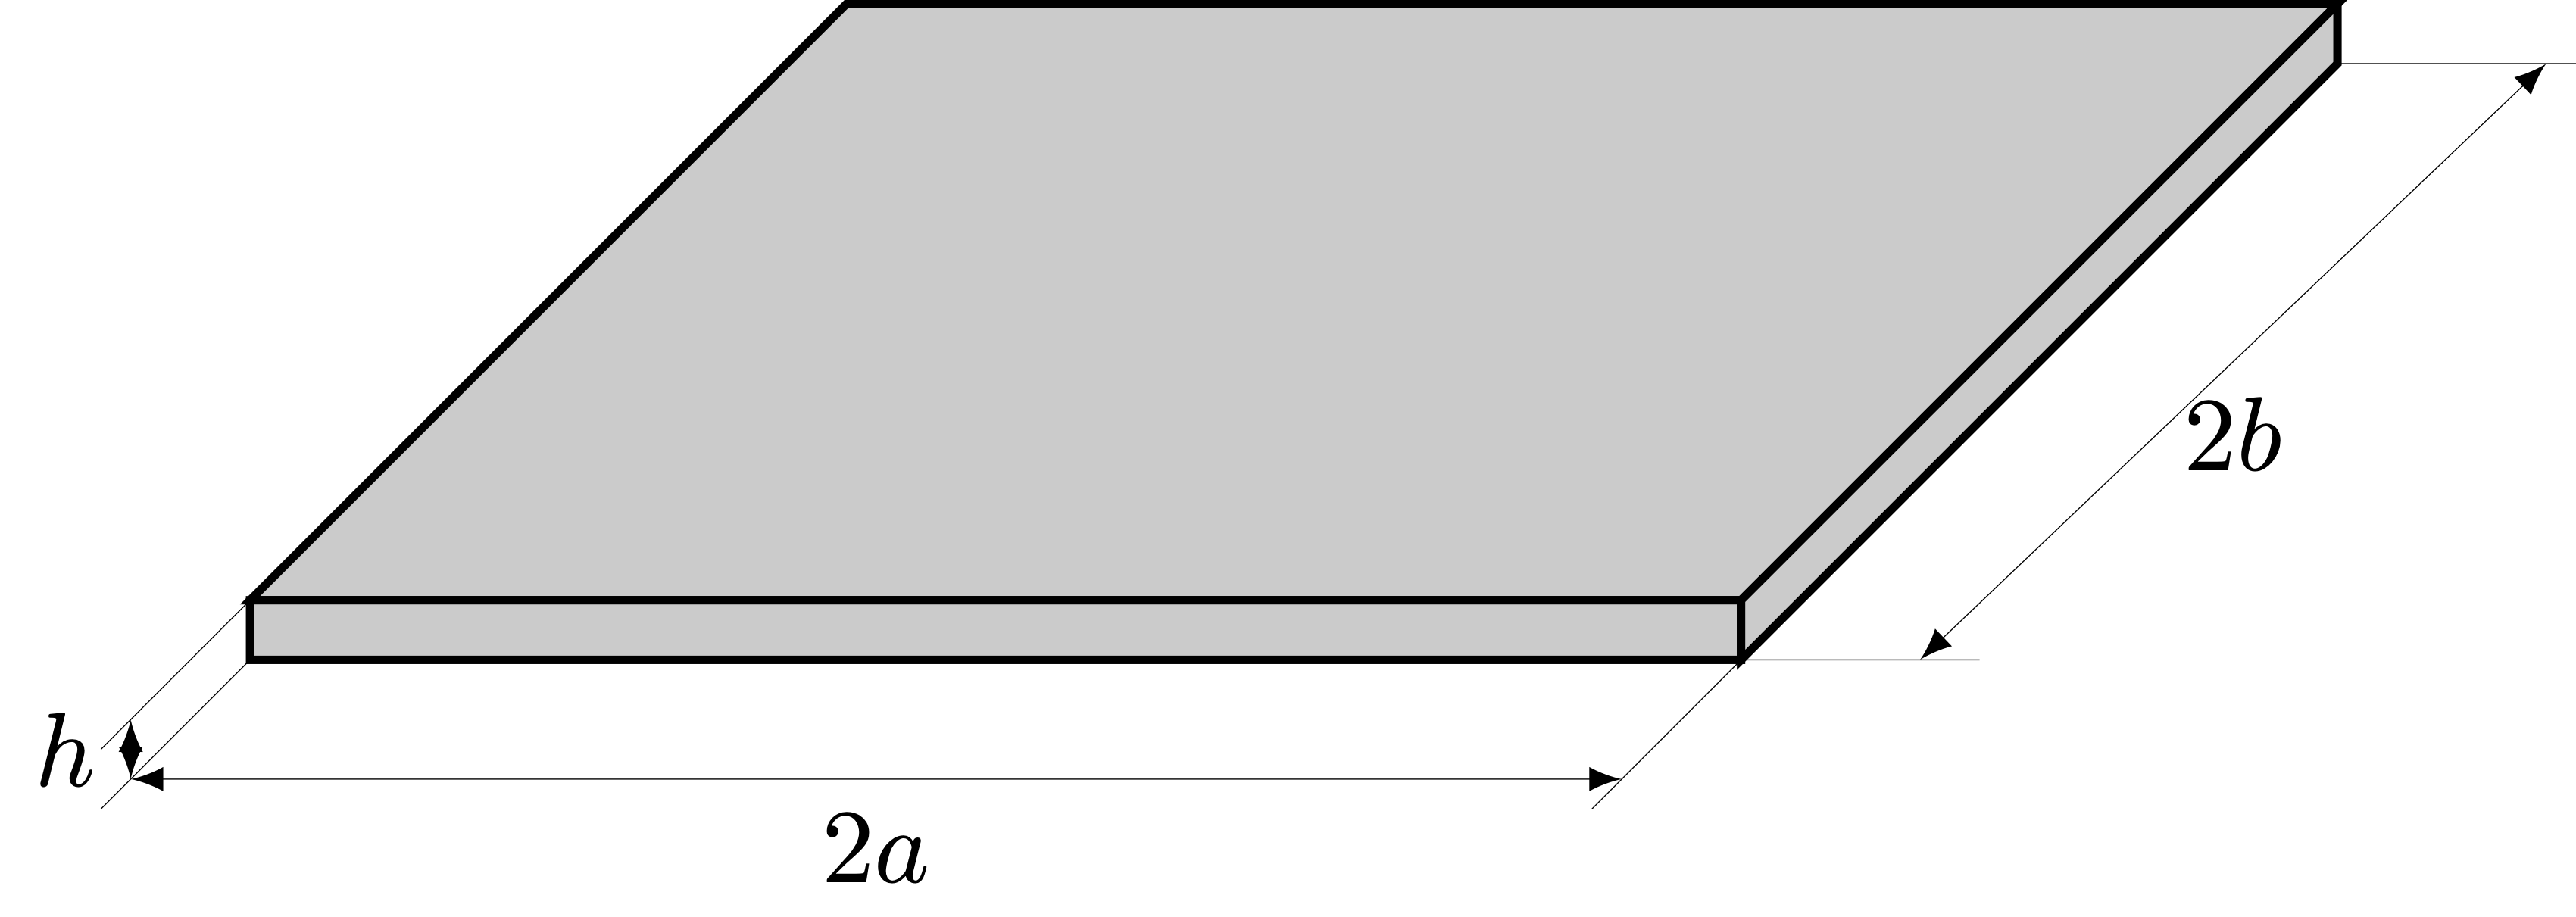
\includegraphics[width=4cm]{../images/plateThin.png}};
    \filldraw (3,0) circle (3pt); % Marker
    \node[align=center] at (3,0.5) {$a\lesssim 0.1h$ \\
      $b\lesssim 0.1h$\\ };
    \node[align=center] at (6,0.7) {Thick \\ plate};
    \node[align=center, below] at (6,-0.2) {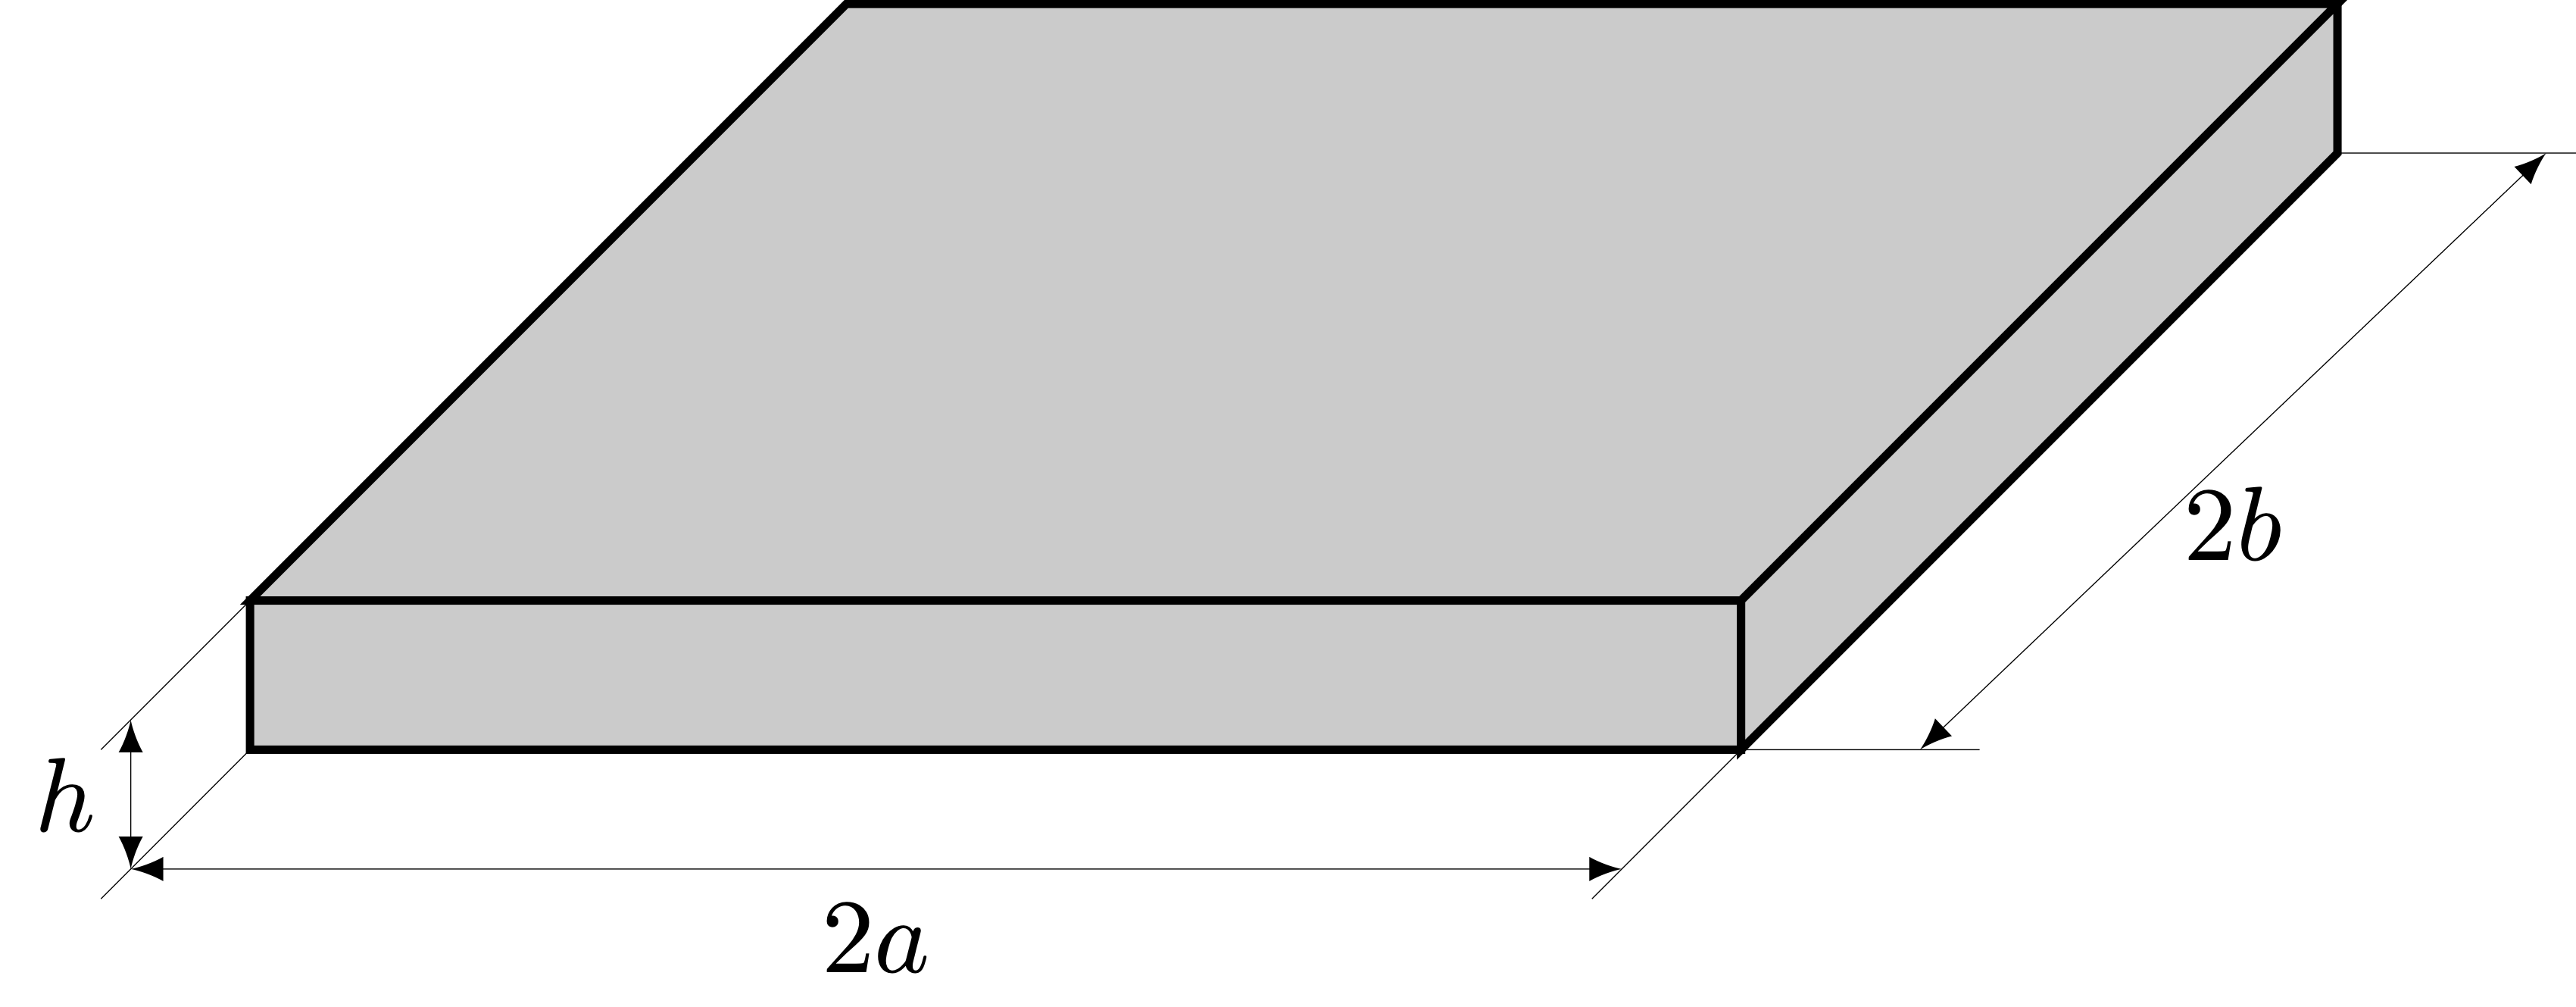
\includegraphics[width=4cm]{../images/plateModThick.png}};
    \filldraw (9,0) circle (3pt); % Marker
    \node[align=center] at (9,0.5) {$a\approx h$ \\
      $b\approx h$\\ }; % Year label
    \node[align=center] at (11,0.7) {3d \\ solid}; % Year label
    \node[align=center,below] at (11,-0.2) {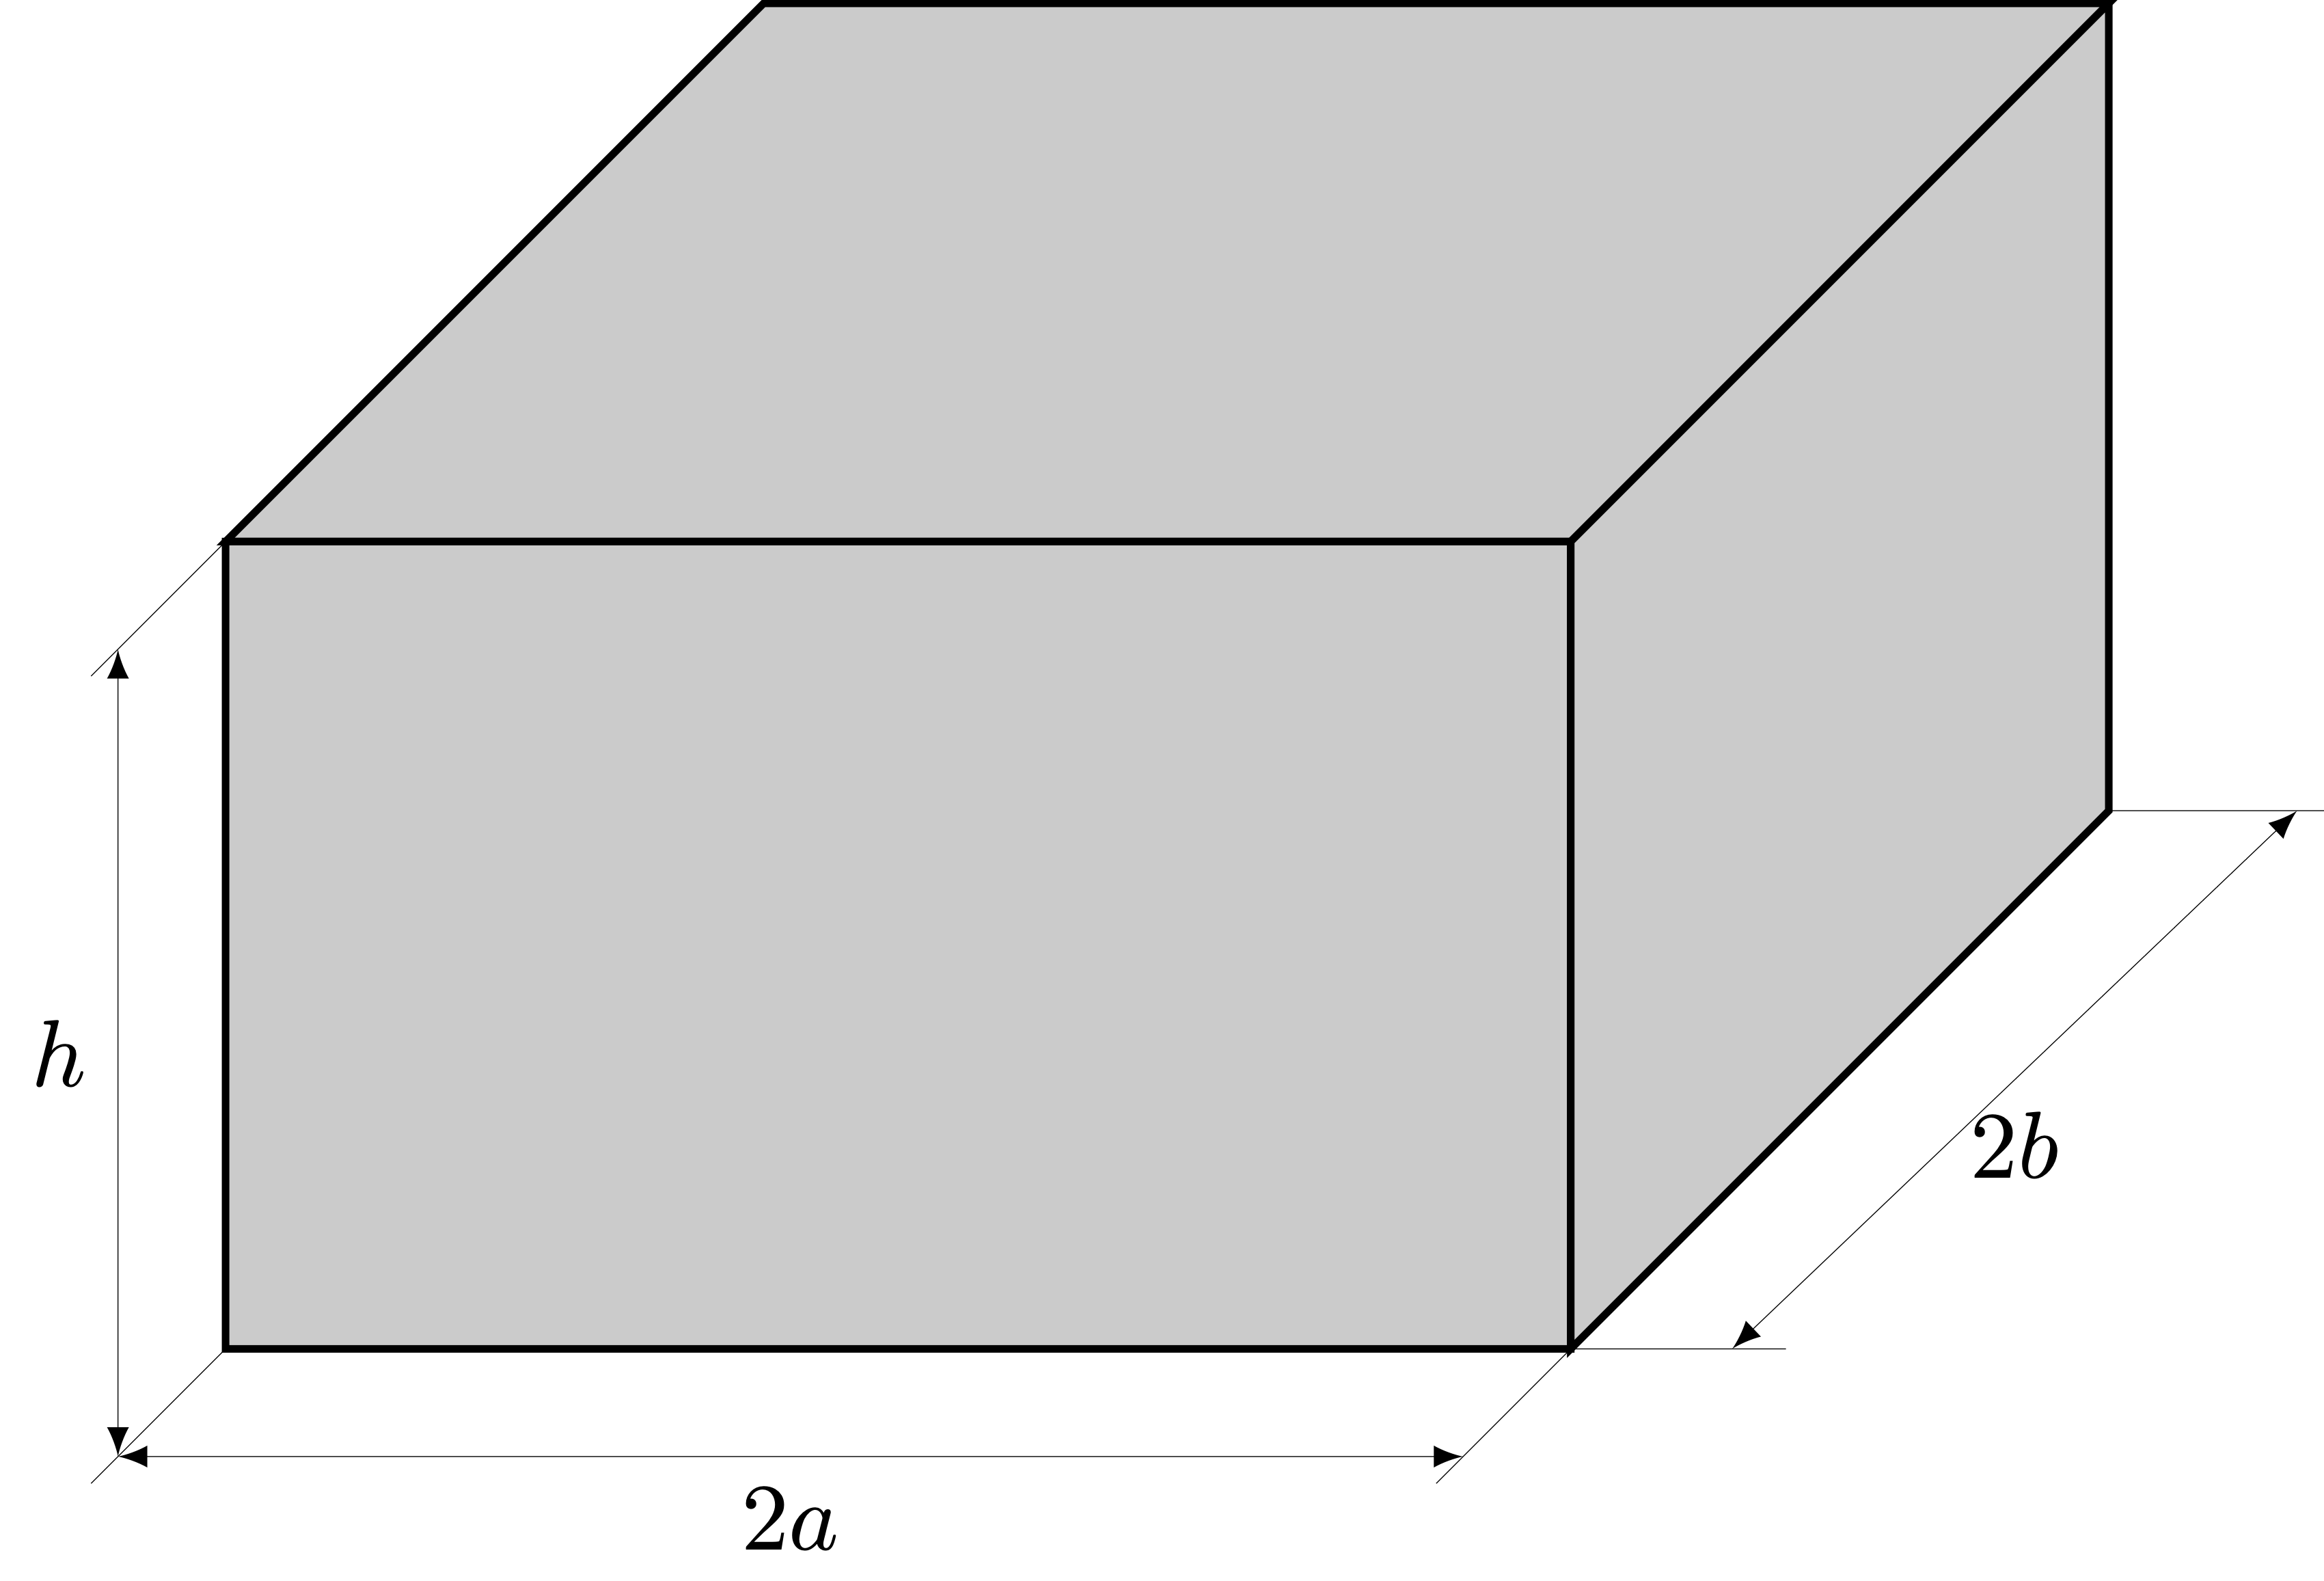
\includegraphics[width=4cm]{../images/plateThick.png}};
  \end{tikzpicture}
\end{frame}

\begin{frame}{Shear deformable plates}
  \begin{itemize}
    \item Thick plate are structures in which shear deformation and rotary inertia effects are important: \emph{transverse shear} becomes an integral part of the formulation.
    \item The material is isotropic, homogenous and linear-elastic according to Hooke's law for a plane stress state where $\sigma_{33}=0$,
    \item Plates carries only transversal loads and in-plane moments that lead to bending deformation of the plate.
  \end{itemize}
  \begin{center}
    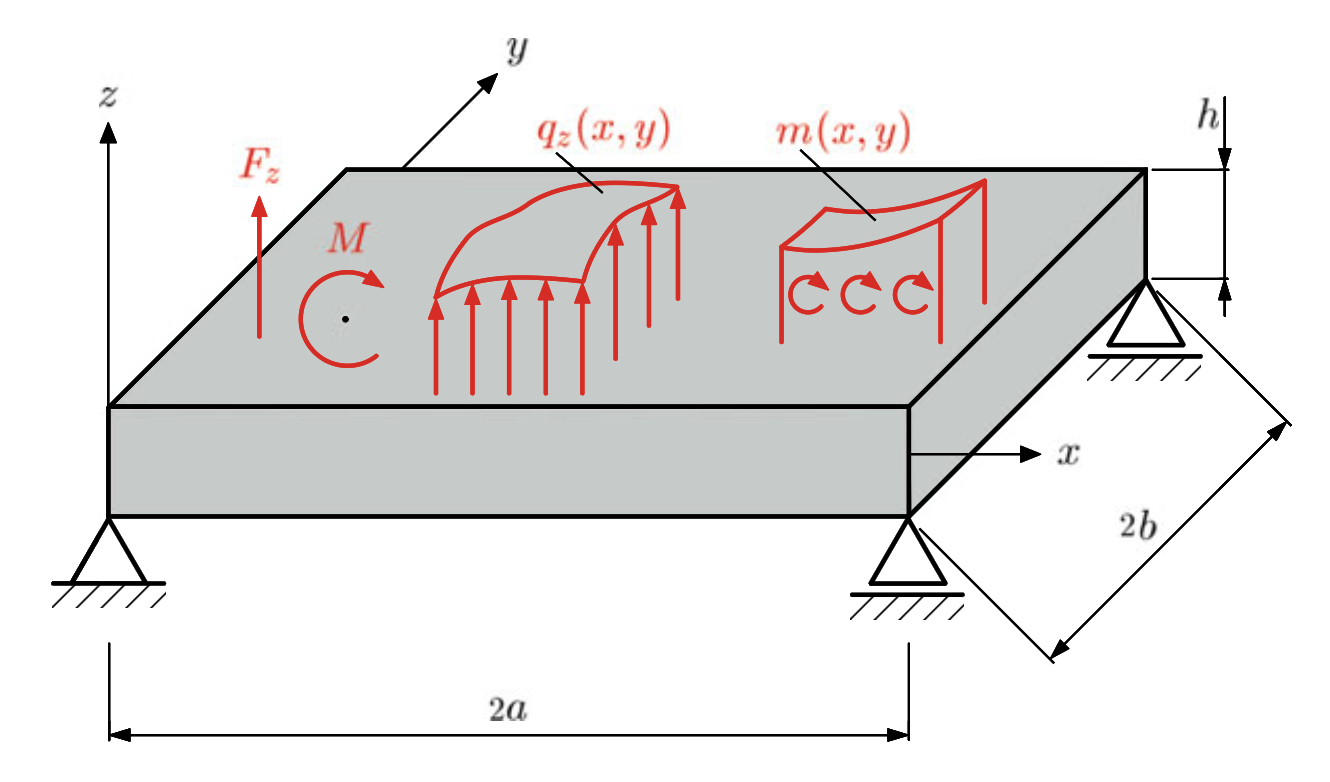
\includegraphics[width=7cm]{../images/PlateThickGenConf.png}
  \end{center}
  \emph{\footnotesize (Credit: (O))}
\end{frame}

\begin{frame}{Reissner-Mindlin assumption}
  \textbf{Planarity of the cross-sectional planes} \\
  Timoshenko's hypothesis is valid, i.e. a cross-sectional plane stays planar and \emph{but not necessarily perpendicular} to the middle surface in the deformed state.
  \begin{center}
    \begin{center}
      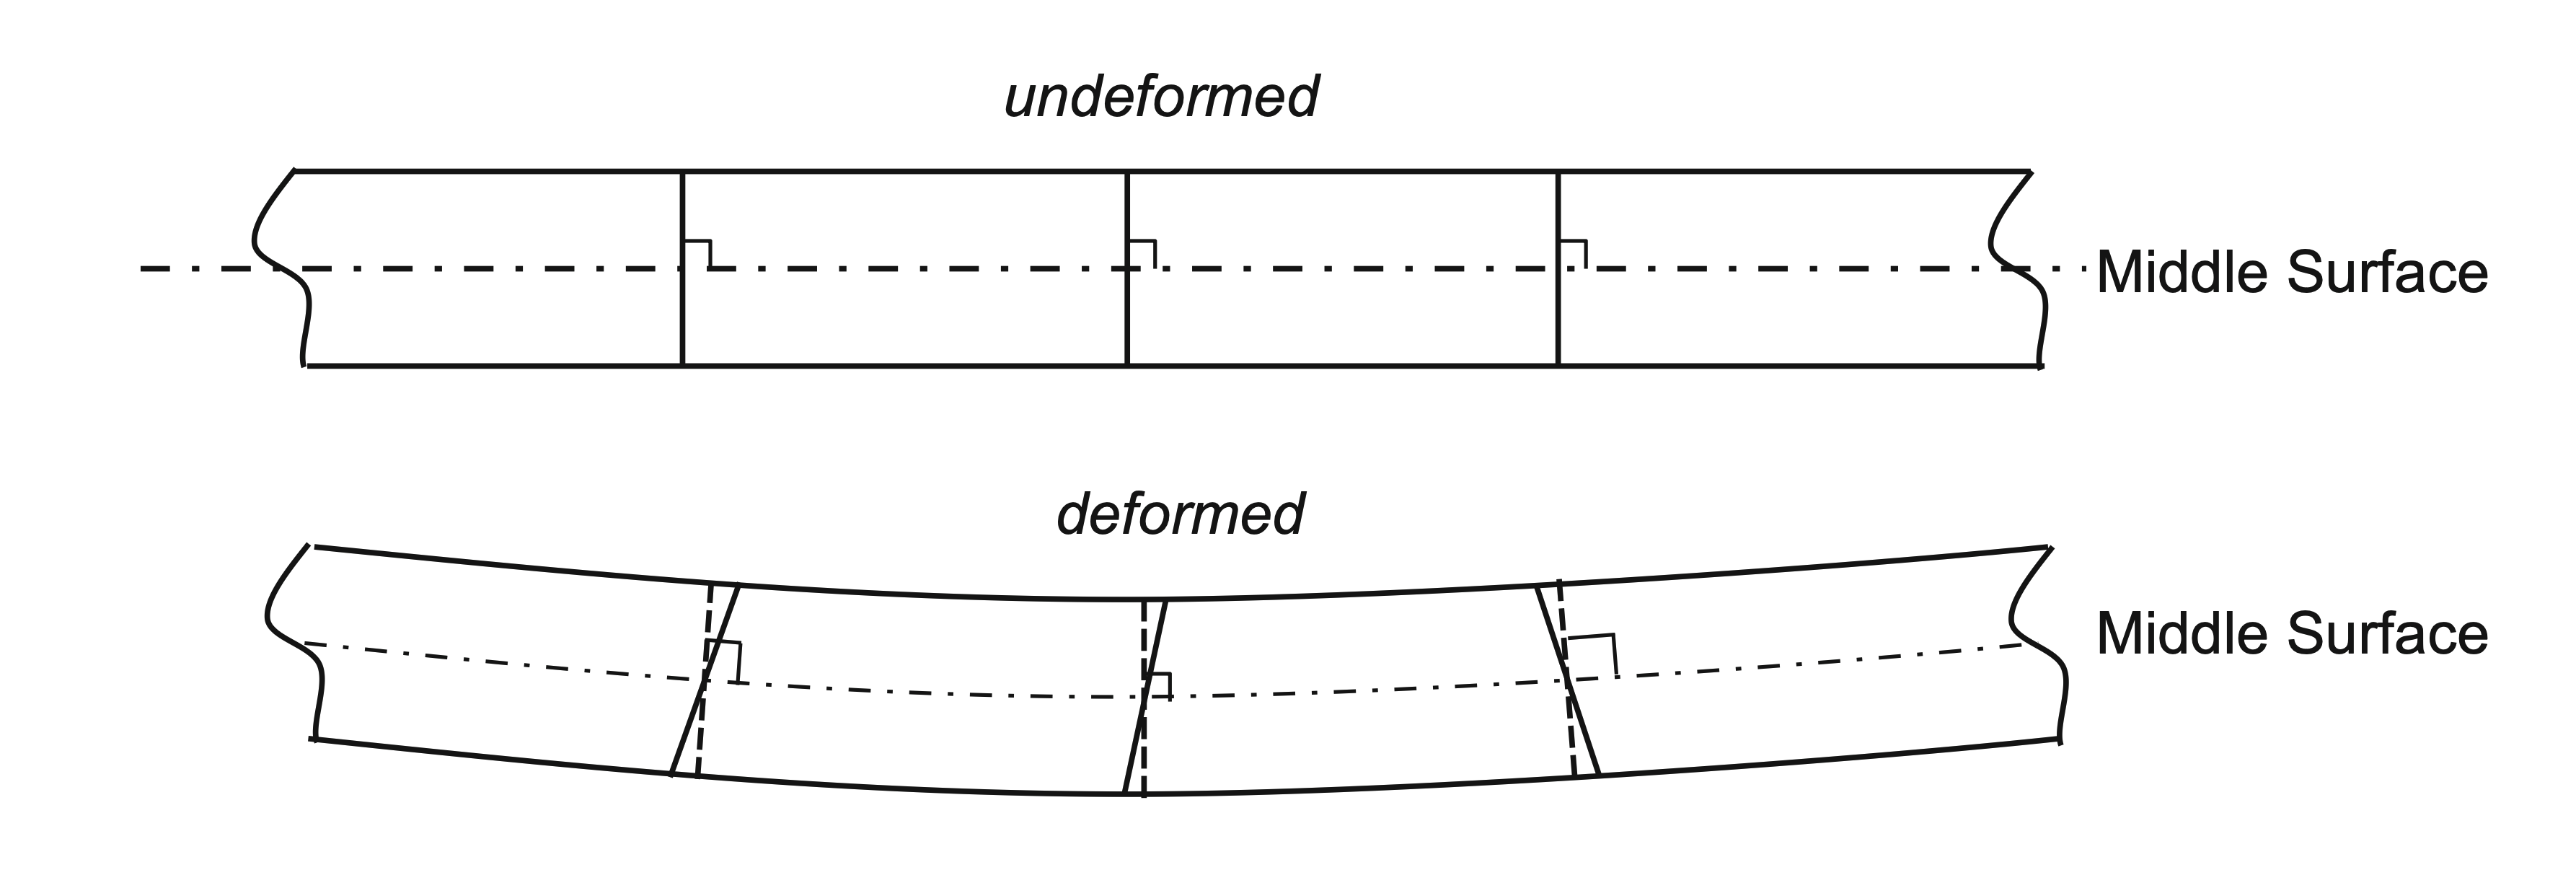
\includegraphics[width=6cm]{../images/ReissnerPlateHp.png}
    \end{center}
  \end{center}
  \begin{tcolorbox}[colback=darkred!10,colframe=darkred!40!black]
    Shear strains $\varepsilon_{13}$ and $\varepsilon_{23}$, due to the distributed shear forces $q_x$ and $q_y$, are \textbf{constant} through the thickness of the plate.
  \end{tcolorbox}
  \emph{\footnotesize (Credit: (N))}
\end{frame}


\begin{frame}{Higher-order deformation theories for plates}
  \begin{columns}
    \begin{column}{0.3\textwidth}
      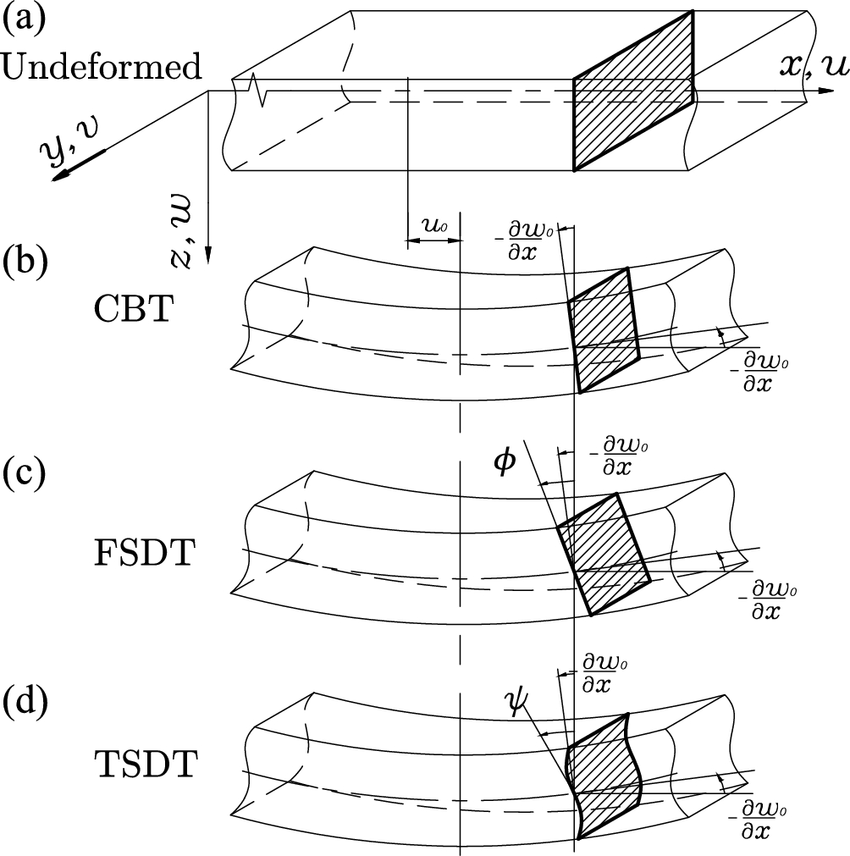
\includegraphics[width=4.5cm]{../images/higherDefTheories.png}
    \end{column}
    \small
    \begin{column}{0.7\textwidth}
      \begin{itemize}
        \item \textbf{Classical plate theory} (Kirchhoff-Love) is a zero-order shear deformation theory.
        \item \textbf{Reissner-Mindlin theory} is a first-order shear deformation theory. Cross-sectional planes remain straight but not necessarily perpendicular to the mid-surface.
              \begin{itemize}
                \item Displacements are linear functions through thickness.
                \item In-plane strains are linear in $z$.
                \item Shear strains are constant in $z$.
              \end{itemize}
        \item  \textbf{Third-order shear deformation theory}: normal cross-sectional planes to the mid-surface can rotate and deform.
              \begin{itemize}
                \item Displacements are cubic functions through thickness.
                \item In-plane strains are cubic in $z$.
                \item Shear strains are quadratic in $z$.
              \end{itemize}
      \end{itemize}
    \end{column}
  \end{columns}
\end{frame}

\begin{frame}{Kinematics assumptions}
  \begin{columns}
    \begin{column}{0.38\textwidth}
      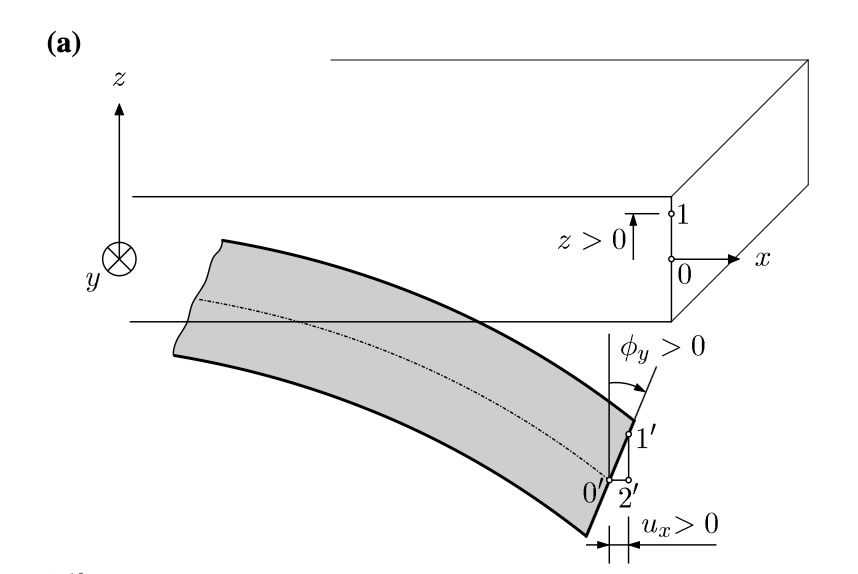
\includegraphics[width=5cm]{../images/plateThickKinematicsXZ.jpeg}
      \vspace{0.2cm}

      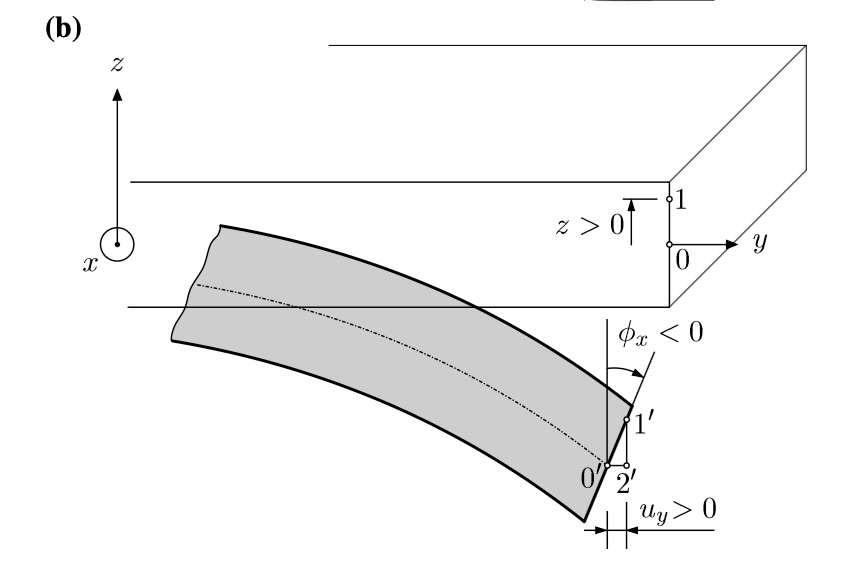
\includegraphics[width=5cm]{../images/plateThickKinematicsXY.jpeg}
    \end{column}

    \begin{column}{0.23\textwidth}
      \begin{block}{}
        \vspace{-0.5cm}
        \begin{align*}
          \phi_2 & \approx\sin(\phi_2)=\frac{u_1}{z}
        \end{align*}
        $$\implies u_1=z \phi_2 $$
      \end{block}
      \vspace{1.5cm}
      \begin{block}{}
        \vspace{-0.5cm}
        \begin{align*}
          \phi_1 & \approx\sin(\phi_1)=-\frac{u_2}{z}
        \end{align*}
        $$\implies u_2=-z \phi_1 $$
      \end{block}
    \end{column}

    \begin{column}{0.4\textwidth}
      \begin{block}{}
        \textbf{Independent variables}:
        \begin{itemize}
          \item Transverse displacement $u_3$
          \item Rotation w.r.t. $Ox$ axis $\phi_1$
          \item Rotation w.r.t. $Oy$ axis $\phi_2$
        \end{itemize}
      \end{block}
      \vspace{0.5cm}
      \footnotesize{Deformation is exaggerated in the figures for better illustration.}
    \end{column}
  \end{columns}
  \vspace{0.3cm}
\end{frame}

\begin{frame}{Strain-displacement relations}
  Using engineering definitions of strain: $\varepsilon_{ii}=\partial_i u_i$ and $\gamma_{ij}=\partial_i u_j+\partial_j u_i$ we obtain:
  \begin{itemize}
    \item \textbf{in-plane or bending strains}:
          $$\underbrace{\begin{bmatrix}
                \varepsilon_{11} \\ \varepsilon_{22} \\ \gamma_{12}
              \end{bmatrix}}_\text{$\boldsymbol{\varepsilon_b}$} = z \underbrace{\begin{bmatrix}
                0 & 0           & \partial_x \\
                0 & -\partial_y & 0          \\
                0 & -\partial_x & \partial_y \\
              \end{bmatrix}}_\text{$\nabla_{b}$} \underbrace{\begin{bmatrix}
                u_3 \\ \phi_1 \\ \phi_2
              \end{bmatrix}}_\text{$\mathbf{u}$},$$
    \item \textbf{transverse shear strains}:
          $$\underbrace{\begin{bmatrix}
                \gamma_{13} \\ \gamma_{23}
              \end{bmatrix}}_\text{$\boldsymbol{\varepsilon_s}$} = \underbrace{\begin{bmatrix}
                \partial_x & 0  & 1 \\
                \partial_y & -1 & 0 \\
              \end{bmatrix}}_\text{$\nabla_{s}$} \underbrace{\begin{bmatrix}
                u_3 \\ \phi_1 \\ \phi_2
              \end{bmatrix}}_\text{$\mathbf{u}$}.$$
  \end{itemize}
  Note that $\varepsilon_{33}=0$ due to the inextensibility of transverse fibers assumption.
\end{frame}

\begin{frame}{Reduction to Kirchhoff-Love plate theory}
  \vspace{0.3cm}
  \begin{columns}
    \begin{column}{0.48\textwidth}
      The transverse shear are exactly equal to the additional rotations of the normal to the reference surface after deformation:
      \begin{align*}
        \gamma_{13} & =\frac{\partial u_3}{\partial x}+\phi_2 \\[5pt]
        \gamma_{23} & =\frac{\partial u_3}{\partial y}-\phi_1
      \end{align*}
    \end{column}

    \begin{column}{0.5\textwidth}
      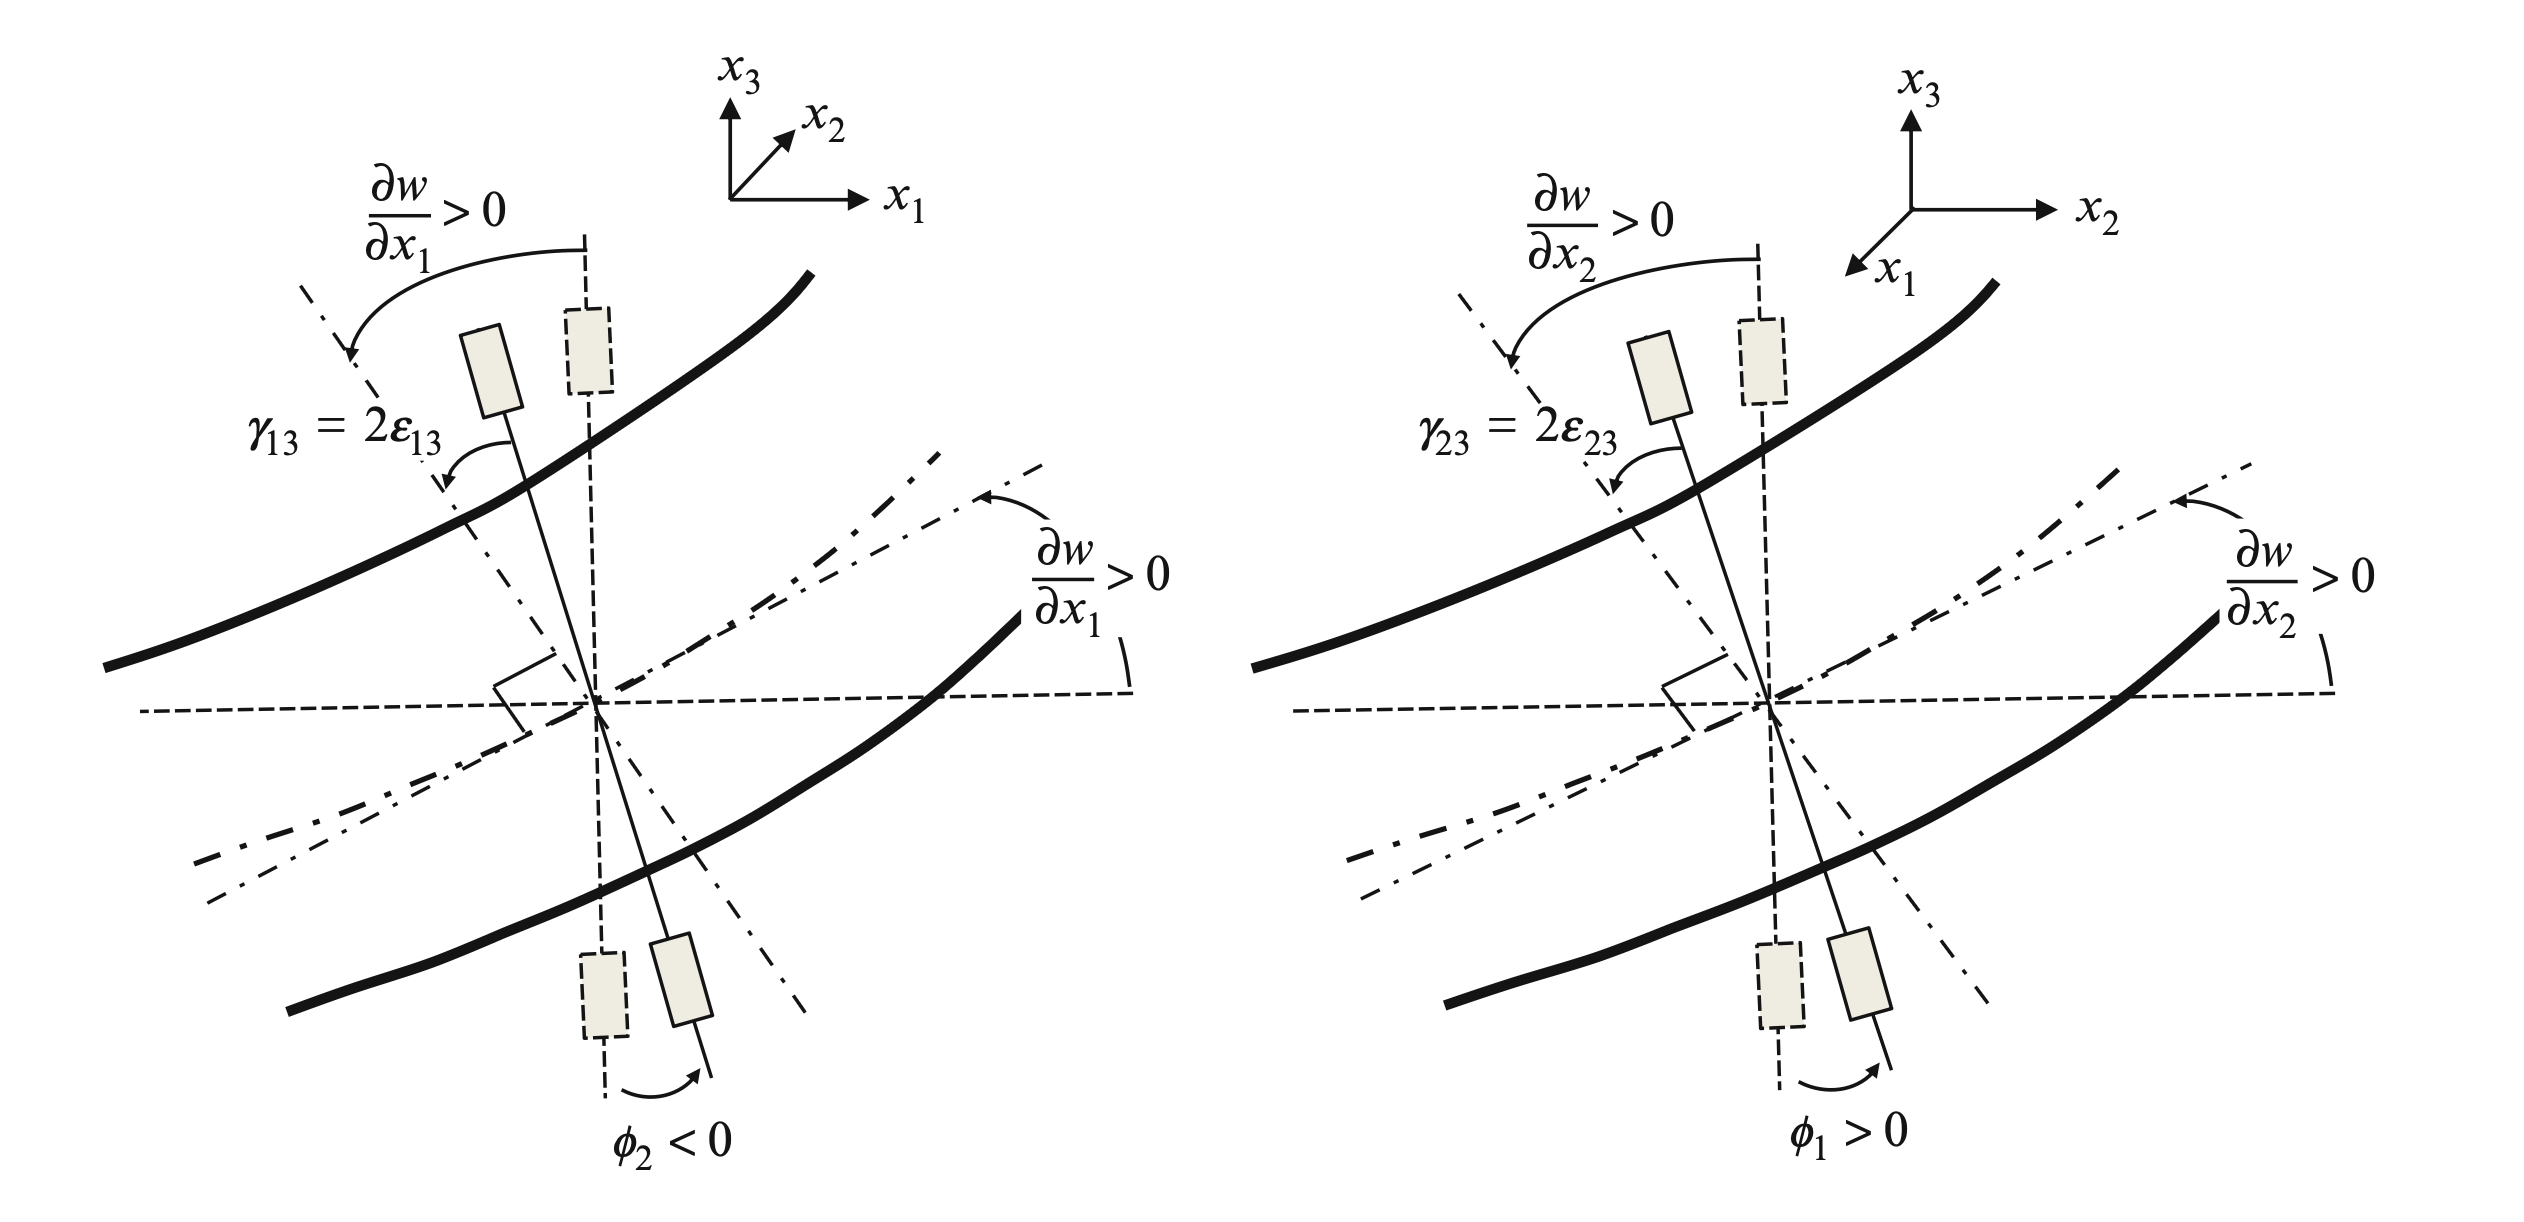
\includegraphics[width=7cm]{../images/transverseShear.png}
    \end{column}
  \end{columns}
  \vspace{0.3cm}
  If the transverse shear strains are negligible, $ \gamma_{13}=0$ and $\gamma_{23}=0$, then, as in the Kirchhoff-Love theory:
  $$\frac{\partial u_3}{\partial x}=-\phi_2\qquad\text{and}\qquad \frac{\partial u_3}{\partial y}=\phi_1 $$
\end{frame}

\begin{frame}{Constitutive equation for isotropic material}
  The constitutive equation for isotropic material is $\overline{\boldsymbol{\sigma}}=\overline{\mathbf C}\overline{\boldsymbol{\varepsilon}}$ where
  \begin{itemize}
    \item \textbf{bending stresses}:
          \[
            \underbrace{\begin{bmatrix}
                \sigma_{11} \\
                \sigma_{22} \\
                \sigma_{12}
              \end{bmatrix}}_\text{$\boldsymbol{\sigma}_b$}
            = \underbrace{
              \frac{E}{1 - \nu^2}
              \begin{bmatrix}
                1   & \nu & 0                 \\
                \nu & 1   & 0                 \\
                0   & 0   & \frac{1 - \nu}{2}
              \end{bmatrix}}_\text{$\mathbf{C}_b$}
            \underbrace{\begin{bmatrix}
                \varepsilon_{11} \\
                \varepsilon_{22} \\
                \gamma_{12}
              \end{bmatrix}}_\text{$\boldsymbol{\varepsilon}_b$},
          \]
    \item \textbf{transverse shear stresses}:
          \[
            \underbrace{\begin{bmatrix}
                \sigma_{13} \\
                \sigma_{23} \\
              \end{bmatrix}}_\text{$\boldsymbol{\sigma}_s$}
            = \underbrace{
              G
              \begin{bmatrix}
                1 & 0 \\
                0 & 1 \\
              \end{bmatrix}}_\text{$\mathbf{C}_s$}
            \underbrace{\begin{bmatrix}
                \gamma_{13} \\
                \gamma_{23} \\
              \end{bmatrix}}_\text{$\boldsymbol{\varepsilon}_s$}.
          \]
  \end{itemize}
  Recall that, for isotropic materials, the shear modulus $G$ is related to Young’s modulus $E$ and Poisson’s ratio $\nu$ by: $G = \frac{E}{2(1 + \nu)}$.
\end{frame}

\begin{frame}{External forces and moments}
  Consider a plate cell of dimensions $dx_1\times dx_2\times h$ that is submitted to external forces, here denoted by $f_3$, and
  area distributed moments $m_1$ and $m_2$ (not shown).
  \begin{center}
    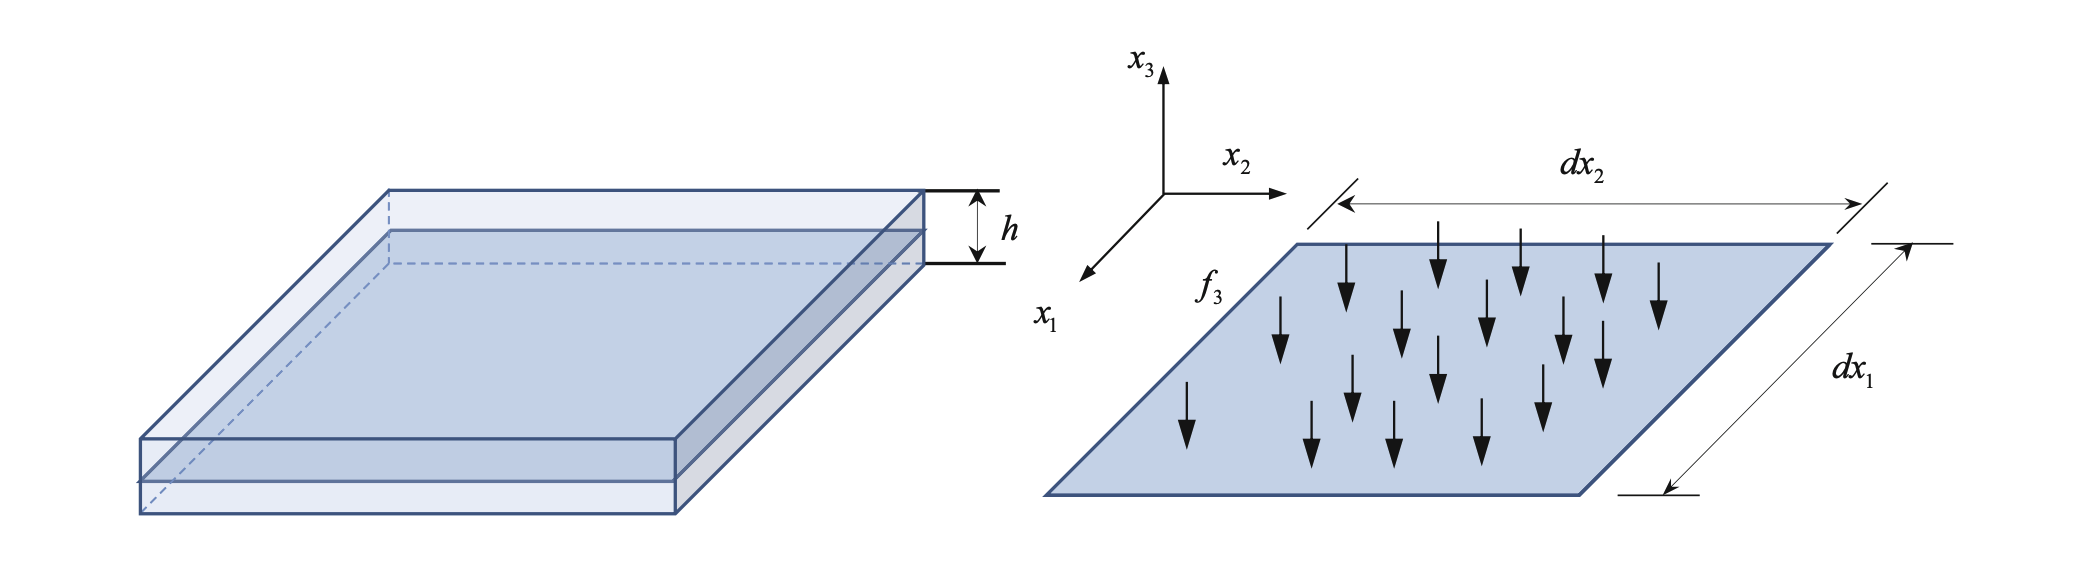
\includegraphics[width=9cm]{../images/plateDynamicEq.png}
  \end{center}
  \begin{columns}
    \begin{column}{0.45\textwidth}
      \begin{center}
        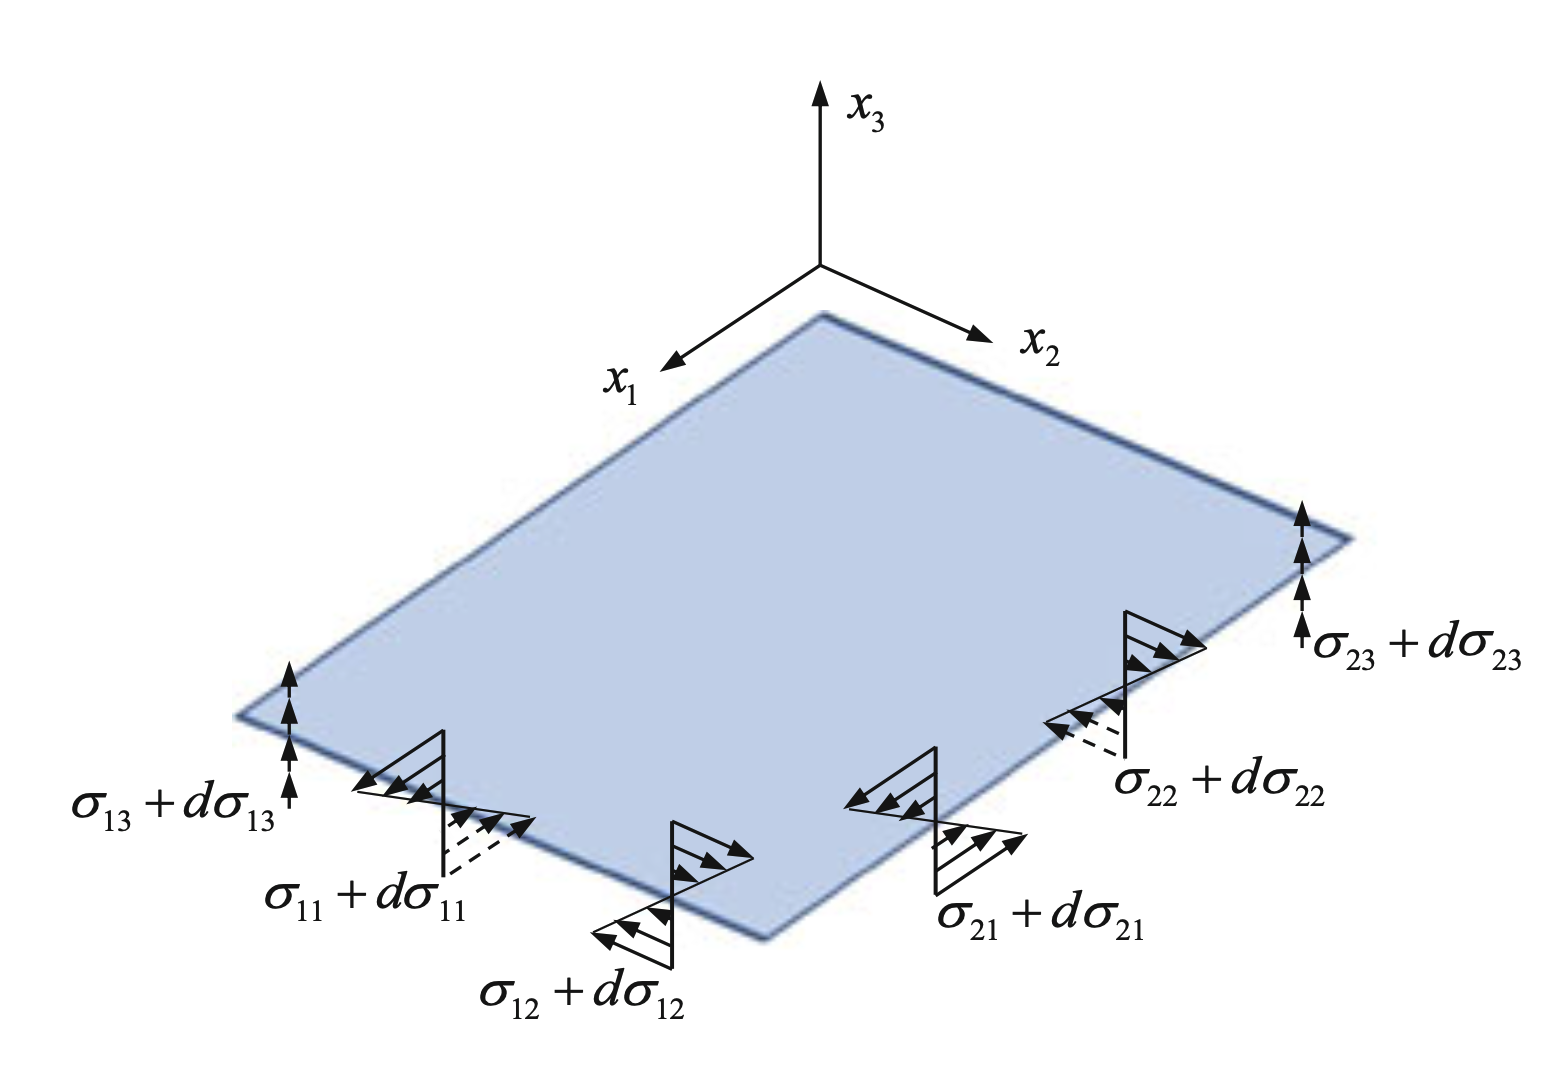
\includegraphics[width=4.5cm]{../images/plateStesses.png}
      \end{center}
    \end{column}

    \begin{column}{0.66\textwidth}
      Normal and shear stresses distributions through the thickness of the plate element:
      \begin{itemize}
        \item linear distributed normal stresses $\sigma_{11}$ and $\sigma_{22}$,
        \item linear distributed shear stresses $\sigma_{12}$ and $\sigma_{21}$,
        \item parabolic distributed transverse shear stresses $\sigma_{13}$ and $\sigma_{23}$.
      \end{itemize}
    \end{column}
  \end{columns}
\end{frame}

\begin{frame}{Normal and shear stresses distributions}

  \begin{itemize}
    \item  Transverse shear strains $\varepsilon_{13}$ and $\varepsilon_{23}$ are constant through the plate thickness (independent of $z$).
    \item Transverse shear stresses $\sigma_{13}$ and $\sigma_{23}$ also have a constant distribution through the plate thickness.
    \item \emph{Transverse shear correction coefficient} $k$: accounts for the discrepancy in transverse shear stress between plate theory and 3D elasticity. It ensures the strain energy from shear stresses in plate theory matches that from 3D elasticity:
          \[
            \underbrace{\begin{bmatrix}
                \sigma_{13} \\
                \sigma_{23} \\
              \end{bmatrix}}_\text{$\boldsymbol{\sigma}_s$}
            = \underbrace{
              kG
              \begin{bmatrix}
                1 & 0 \\
                0 & 1 \\
              \end{bmatrix}}_\text{$\mathbf{C}_s$}
            \underbrace{\begin{bmatrix}
                \gamma_{13} \\
                \gamma_{23} \\
              \end{bmatrix}}_\text{$\boldsymbol{\varepsilon}_s$}.
          \]
  \end{itemize}
  \begin{block}{}
    \centering \textbf{For homogeneous isotropic rectangular plates : $k=5/6$.}
  \end{block}
\end{frame}

\begin{frame}{Moments and shear forces}
  \begin{columns}
    \begin{column}{0.45\textwidth}
      \begin{center}
        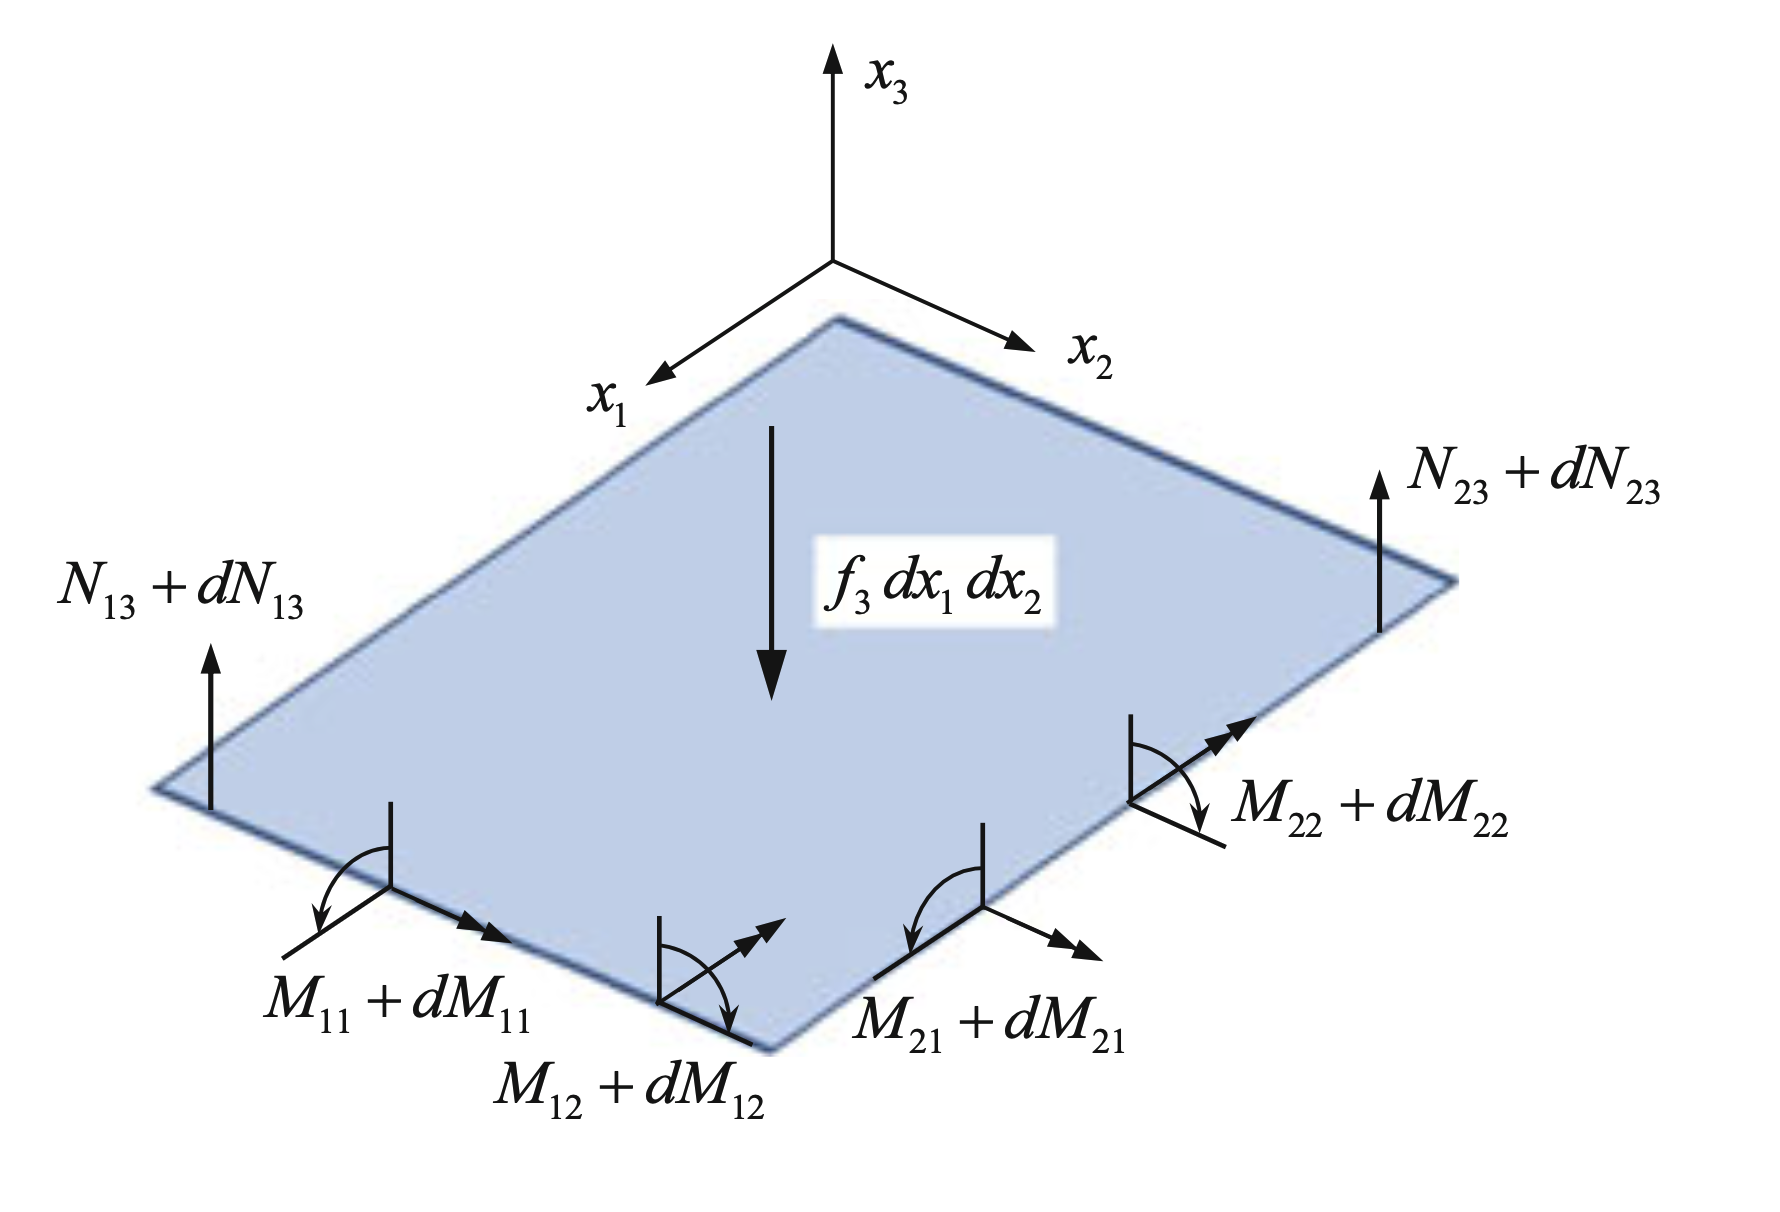
\includegraphics[width=4.5cm]{../images/plateMoments.png}
      \end{center}
    \end{column}

    \begin{column}{0.66\textwidth}
      Moments and shear forces acting along the edge of the plate:
      \begin{itemize}
        \item bending moments $M_{11}$ and $M_{22}$,
        \item twisting moment $M_{12}$,
        \item shear forces $N_{13}$ and $N_{23}$.
      \end{itemize}
    \end{column}
  \end{columns}
  \vspace{0.3cm}
  \begin{align*}
    \mathbf{M} & =
    \begin{bmatrix}
      M_{11} \\
      M_{22} \\
      M_{12}
    \end{bmatrix}
    =
    \int_{-\frac{h}{2}}^{\frac{h}{2}} x_3 \, \boldsymbol{\sigma}_b \, dx_3
    =
    \boldsymbol{C}_b\nabla_b\mathbf u\int_{-\frac{h}{2}}^{\frac{h}{2}} x_3^2  \, dx_3 =\underbrace{\frac{h^3}{12}\boldsymbol{C}_b}_\text{$\overline{\boldsymbol{C}_b}$}\nabla_b\mathbf u \\
    \mathbf{N} & =
    \begin{bmatrix}
      N_{13} \\
      N_{23} \\
    \end{bmatrix}
    =
    \int_{-\frac{h}{2}}^{\frac{h}{2}} \boldsymbol{\sigma}_s
    \, dx_3
    =\underbrace{h\boldsymbol{C}_s}_\text{$\overline{\boldsymbol{C}_s}$}\nabla_s\mathbf u
  \end{align*}
\end{frame}

{\setbeamercolor{background canvas}{bg=darkred}
\setbeamercolor{block body}{bg=darkred,fg=white}
\setbeamercolor{itemize item}{fg=white}
\setbeamercolor{itemize/enumerate body}{fg=white}
\color{white}
\begin{frame}{Moments and shear forces}
  \begin{block}{}
    In matrix form:
    $$\begin{bmatrix}
        \mathbf{M} \\ \mathbf{N}
      \end{bmatrix}=\underbrace{\begin{bmatrix}
          \overline{\boldsymbol{C}_b} & \mathbf 0                   \\
          \mathbf 0                   & \overline{\boldsymbol{C}_s}
        \end{bmatrix}}_\text{$\overline{\boldsymbol{C}}$}\underbrace{\begin{bmatrix}
          \nabla_b \\ \nabla_s
        \end{bmatrix}}_\text{$\nabla_r$}\mathbf u,$$
    Here
    $$\nabla_r=\begin{bmatrix}
        \nabla_b \\ \nabla_s
      \end{bmatrix}=\begin{bmatrix}
        0          & 0           & \partial_x \\
        0          & -\partial_y & 0          \\
        0          & -\partial_x & \partial_y \\
        \partial_x & 0           & 1          \\
        \partial_y & -1          & 0          \\
      \end{bmatrix},$$
    $$ \overline{\boldsymbol{C}_b}=\frac{Eh^3}{12(1 - \nu^2)}\begin{bmatrix}
        1   & \nu & 0                 \\
        \nu & 1   & 0                 \\
        0   & 0   & \frac{1 - \nu}{2}
      \end{bmatrix}\qquad\text{and}\qquad \overline{\boldsymbol{C}_s}= \frac{Ekh}{2(1 + \nu)}\begin{bmatrix}
        1 & 0 \\
        0 & 1 \\
      \end{bmatrix}.$$
  \end{block}
\end{frame}
}

\begin{frame}{Dynamic equilibrium equations}
  \begin{itemize}
    \item Equilibrium condition for the vertical forces:
          $$\frac{\partial N_{13}}{\partial x_1}+\frac{\partial N_{23}}{\partial x_2}+f_3=\rho h \ddot{u}_3$$
    \item Equilibrium of moments:
          $$\frac{\partial M_{11}}{\partial x_1}+\frac{\partial M_{12}}{\partial x_2}+m_2-N_{13}=\rho \frac{h^3}{12} \ddot{\phi}_2$$
          $$\frac{\partial M_{22}}{\partial x_2}+\frac{\partial M_{12}}{\partial x_1}-m_1-N_{23}=-\rho \frac{h^3}{12} \ddot{\phi}_1$$
  \end{itemize}
\end{frame}

\begin{frame}{Dynamic equilibrium equation}
  \begin{block}{}
    In matrix form:
    $$\underbrace{\begin{bmatrix}
          0          & 0           & 0           & \partial_x & \partial_y \\
          0          & -\partial_y & -\partial_x & 0          & 1          \\
          \partial_x & 0           & \partial_y  & -1         & 0          \\
        \end{bmatrix}}_\text{$\nabla_m^T$} \begin{bmatrix}
        \mathbf{M} \\ \mathbf{N}
      \end{bmatrix}+\underbrace{\begin{bmatrix}
          f_3 \\ m_1 \\ m_2
        \end{bmatrix}}_\text{$\mathbf f$}=\underbrace{\begin{bmatrix}
          \rho h & 0           & 0           \\
          0      & \rho h^3/12 & 0           \\
          0      & 0           & \rho h^3/12 \\
        \end{bmatrix}}_\text{$\mathbf I$} \ddot{\mathbf{u}}$$
    \vspace{-0.3cm}
    \begin{itemize}
      \item  $\mathbf I$ mass moment of inertia matrix:
            \begin{itemize}
              \item $\rho h$ translational inertia (in the transverse $x_3$-direction),
              \item  $\rho h^3/12$: rotational inertia (about the in-plane $x_1$- and $x_2$-axes).
            \end{itemize}
      \item  $\mathbf f$  applied forces and moments.
      \item  Linear elastic stress-strain relation and the constitutive relation:
            $$\begin{bmatrix}
                \mathbf{M} \\ \mathbf{N}
              \end{bmatrix}=\overline{\boldsymbol{C}}\nabla_r\mathbf u$$
    \end{itemize}

  \end{block}
\end{frame}

{\setbeamercolor{background canvas}{bg=darkred}
\setbeamercolor{block body}{bg=darkred,fg=white}
\setbeamercolor{itemize item}{fg=white}
\setbeamercolor{itemize/enumerate body}{fg=white}
\color{white}
\begin{frame}{Strong form for Reissner-Mindlin plate bending}
  \begin{block}{}
    Let $\Omega=[-a,a]\times[-b,b]$ be a rectangular plate. Find the transverse displacement $u_{3}\in C^2(\Omega\times[0,T])$ and the rotations $\phi_1,\ \phi_2\in C^2(\Omega\times[0,T])$ such that
    $$
      \nabla_m^T \overline{\boldsymbol{C}}\nabla_r\mathbf{u}+\mathbf f=\mathbf{I} \ddot{\mathbf u} \qquad \text{  on  }\Omega\times]0,T[
    $$
    \vspace{-0.5cm}
    \begin{columns}
      \begin{column}{0.55\textwidth}
        \begin{itemize}
          \item boundary conditions (simply supported):
                \vspace{-0.2cm}
                \[
                  \begin{aligned}
                     & u_3 = 0\qquad   & \text{in }\partial\Omega\times]0,T[   \\
                     & \phi_2 =0\qquad & \text{in }\partial\Omega_1\times]0,T[ \\
                     & \phi_1 =0\qquad & \text{in }\partial\Omega_2\times]0,T[
                  \end{aligned}
                \]
          \item
                initial conditions:
                \vspace{-0.2cm}
                \[
                  \begin{aligned}
                     & \color{orange}{\mathbf u(\cdot, 0) =  \mathbf u_0 \quad \text{in }\Omega}      \\
                     & \color{orange}{\dot{\mathbf u}(\cdot, 0) = \mathbf v_0 \quad \text{in }\Omega} \\
                  \end{aligned}
                \]
        \end{itemize}
      \end{column}

      \begin{column}{0.38\textwidth}
        \begin{center}
          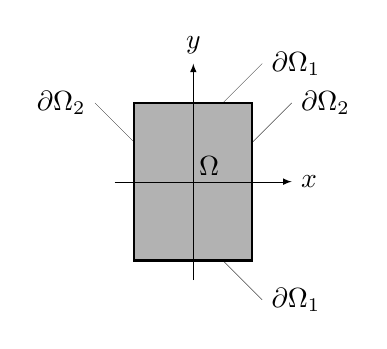
\begin{tikzpicture}[scale=0.5]
            \def\a{3}
            \def\b{4}
            % Draw the rectangle
            \filldraw[fill=gray!60, draw=black,thick] (0,0) rectangle (\a,\b);
            %axis
            \draw[-latex,ultra thin] (-0.5,\b/2) -- (\a+1,\b/2) node[right]{$x$};
            \draw[-latex, ultra thin] (\a/2,-0.5) -- (\a/2,\b+1)node[above]{$y$};
            % Omega
            \node at (\a/2+0.4,\b/2+0.4) {$\Omega$};
            \draw[ultra thin] (3*\a/4,\b) -- (3*\a/4+1,\b+1) node[right]{$\partial\Omega_1$};
            \draw[ultra thin] (\a,3*\b/4) -- (\a+1,3*\b/4+1) node[right]{$\partial\Omega_2$};
            \draw[ultra thin] (3*\a/4,0) -- (3*\a/4+1,-1) node[right]{$\partial\Omega_1$};
            \draw[ultra thin] (0,3*\b/4) -- (-1,3*\b/4+1) node[left]{$\partial\Omega_2$};
          \end{tikzpicture}
        \end{center}
      \end{column}
    \end{columns}
  \end{block}
\end{frame}
}

\begin{frame}{Strong form for Reissner-Mindlin plate bending}
  Expanding the strong form, for isotropic material, the dynamic equation in matrix form results in the following system of partial differential equations:
  \begin{align*}
     & \left[
      \begin{array}{ccc}
        D_s \left( \partial^2_{xx} +\partial^2_{yy}  \right) & -D_s\partial_{y}                                                             & D_s\partial_{x}                                                              \\[5pt]
        D_s \partial_{y}                                     & D_b \left( \frac{1 - \nu}{2} \partial^2_{xx}  +\partial^2_{yy} \right) - D_s & -\frac{1 + \nu}{2} D_b \partial^2_{xy}                                       \\[5pt]
        -D_s\partial_{x}                                     & -\frac{1 + \nu}{2} D_b \partial^2_{xy}                                       & D_b \left(\partial^2_{xx} + \frac{1 - \nu}{2} \partial^2_{yy}  \right) - D_s
      \end{array}
      \right]
    \left[
      \begin{array}{c}
        u_3    \\[5pt]
        \phi_1 \\[5pt]
        \phi_2
      \end{array}
      \right]
    +         \\
     & +
    \left[
      \begin{array}{c}
        f_3 \\
        m_1 \\
        m_2
      \end{array}
      \right]
    =
    \left[
      \begin{array}{c}
        \rho h\, \ddot{u}_3         \\
        \rho h^3/12\, \ddot{\phi}_1 \\
        \rho h^3/12\, \ddot{\phi}_2
      \end{array}
      \right]
  \end{align*}
  where $D_s=khG$, and $D_b=\frac{Eh^3}{12(1-\nu^2)}$.
\end{frame}

{\setbeamercolor{background canvas}{bg=darkred}
\setbeamercolor{block body}{bg=darkred,fg=white}
\setbeamercolor{itemize item}{fg=white}
\setbeamercolor{itemize/enumerate body}{fg=white}
\color{white}
\begin{frame}{Weak form for Reissner-Mindlin plate bending}
  The weak form consists of finding the transverse displacement $u_{3}\in \mathcal U$ and the rotations $\phi_1,\ \phi_2\in \mathcal U$ such that the following equation is satisfied for every $\bolddelta\mathbf u\in \mathcal V$:
  \begin{block}{}
    \[
      \int_\Omega \, (\nabla_r \bolddelta\mathbf{u})^T\, \overline{\mathbf C} \, \nabla_r \mathbf u \, d\Omega + \int_\Omega \bolddelta\mathbf u^T\, \mathbf I\, \ddot{\mathbf u} \, d\Omega = \int_\Omega \bolddelta\mathbf u^T\mathbf f \, d\Omega
    \]
  \end{block}

  \vspace{-0.5cm}
  \begin{align*}
    \mathcal U & =\big\{\mathbf u(\cdot,t)\in H^1(\Omega)\ |\ u_3(\cdot,t)=0\text{ in } \partial\Omega,\   \phi_1(\cdot,t)=0\text{ in } \partial\Omega_2,\ \phi_2(\cdot,t)=0\text{ in } \partial\Omega_1 \big\} \\
    \mathcal V & =\big\{\bolddelta\mathbf u\in H^1(\Omega)\ |\ \delta u_3=0\text{ in } \partial\Omega,\  \delta\phi_1=0\text{ in } \partial\Omega_2,\ \delta\phi_2=0\text{ in } \partial\Omega_1\big\}
  \end{align*}
\end{frame}
}
\section{Thick plate bending elements}

\begin{frame}{Overview of thick plate bending elements}
  Numerous finite elements for plate bending have been developed: \textbf{more than 88 distinct types} (thick and thin combined) can be identified.
  \begin{center}
    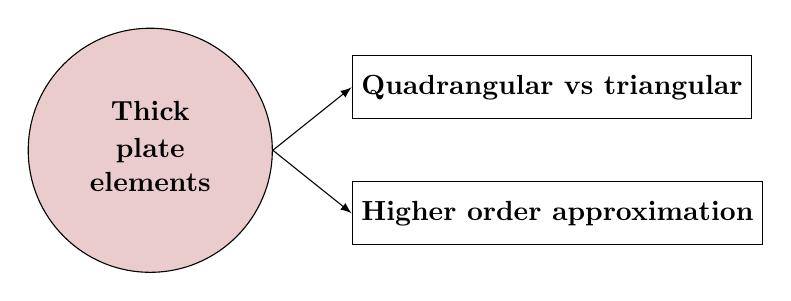
\begin{tikzpicture}
      \node[circle, draw, minimum size=3.1cm, fill=darkred!20] (circle) at (0,0){};
      \node at (0,0.5) {\textbf{Thick}};
      \node at (0,0) {\textbf{plate}};
      \node at (0,-0.4) {\textbf{elements}};
      % Define the list of polynomial degrees
      \foreach \i/\txt in {1/Quadrangular vs triangular, 3/Higher order approximation} {
          % Compute y-shift to center the list
          \pgfmathsetmacro{\yshift}{(2-\i) * 0.8}
          % Draw rectangles with text
          \node[draw, minimum width=2cm, minimum height=0.8cm, right=1cm of circle, yshift=\yshift cm] (box\i) {\textbf{\txt}};
          % Draw connecting arrows
          \draw[-latex] (circle.east) -- (box\i.west);
        }
    \end{tikzpicture}
  \end{center}
  \begin{itemize}
    \item  1977 - \textbf{Hughes-Taylor-Kanoknukulcha element (HTK)}: 12 dofs quadrangular, thick plate bending element.
  \end{itemize}
\end{frame}

\begin{frame}{Generalized displacements approximation}
  \begin{block}{}
    Since the rotations $\phi_1$ and $\phi_2$ are defined independently of the transversal displacement $u_3$, the discretization procedure uses 2D bilinear finite elements.
  \end{block}
  \vspace{-0.2cm}
  \begin{align*}
    {}^eu_3(x,y,t)    & = \sum_{i=1}^{4}{}^eh_{i}(x,y){}^ed^{i}(t)        \\[5pt]
    {}^e\phi_1(x,y,t) & = \sum_{i=1}^{4}{}^eh_{i}(x,y){}^e\theta^{i}_1(t) \\[5pt]
    {}^e\phi_2(x,y,t) & = \sum_{i=1}^{4}{}^eh_{i}(x,y){}^e\theta^{i}_2(t)
  \end{align*}
  The shape functions ${}^e h_i$ are bilinear Lagrangian functions defined over the element.
\end{frame}

\begin{frame}{Generalized displacements approximation}
  \begin{block}{}
    \vspace{-0.4cm}
    \begin{align*}
      {}^e \mathbf u^{h}(\mathbf x,t) & ={}^e \mathbf H(\mathbf x){}^e\mathbf q(t) = \sum_{i=1}^{4}{}^eh_{i}(\mathbf x){}^e\mathbf q^{i}(t)
    \end{align*}
  \end{block}
  \begin{itemize}
    \item ${}^e\mathbf H(\mathbf x)$ is a $3\times 12$ matrix of \textbf{shape functions}:
          $$
            {}^e\mathbf H
            =\left[
              \begin{array}{c;{2pt/2pt}c;{2pt/2pt}c;{2pt/2pt}c}
                h_{1}\mathbf I & h_{2}\mathbf I & h_{3}\mathbf I & h_{4}\mathbf I \\
              \end{array} \right] = \begin{bmatrix}
              {}^eh_1 & 0       & 0       &       & {}^eh_{4} & 0         & 0         \\
              0       & {}^eh_1 & 0       & \dots & 0         & {}^eh_{4} & 0         \\
              0       & 0       & {}^eh_1 &       & 0         & 0         & {}^eh_{4} \\
            \end{bmatrix}
          $$
          $\mathbf I$ is the $3\times 3$ identity matrix.
    \item ${}^e\mathbf q^i(t)=\begin{bmatrix}
              {}^e d^{i}(t) \\ {}^e \theta^{i}_1(t) \\ {}^e \theta^{i}_2(t)
            \end{bmatrix}$ is the vector of generalized displacements of node $i$.
  \end{itemize}
\end{frame}

\begin{frame}{Elementary stiffness matrix}
  \begin{block}{}
    $${}^e\mathbf K=\int_{{}^e\Omega} {}^e\mathbf B^T\overline{\mathbf C}{}^e\mathbf B \, d\Omega$$
  \end{block}
  \begin{itemize}
    \item Elementary deformation matrix ($5\times 12$):
          $${}^e\mathbf B=\nabla_r {}^e\mathbf H=\left[
              \begin{array}{c;{2pt/2pt}c;{2pt/2pt}c}
                \nabla_r {}^eh_1 & \dots & \nabla_r {}^eh_{4}
              \end{array} \right]=\left[
              \begin{array}{c;{2pt/2pt}c;{2pt/2pt}c}
                \nabla_b {}^eh_1 & \dots & \nabla_b {}^eh_{4} \\
                \nabla_s {}^eh_1 & \dots & \nabla_s {}^eh_{4} \\
              \end{array} \right]=\left[
              \begin{array}{c}
                \nabla_b {}^e\mathbf H \\
                \nabla_s {}^e\mathbf H \\
              \end{array} \right]$$
  \end{itemize}
  \begin{block}{}
    \vspace{0.2cm}
    \begin{itemize}
      \item Bending strain-displacement matrix:
            ${}^e\mathbf B_b=\nabla_b {}^e\mathbf H$.
      \item Shear strain-displacement matrix:
            ${}^e\mathbf B_s=\nabla_s {}^e\mathbf H$.
            \vspace{0.2cm}
    \end{itemize}
  \end{block}
  \begin{itemize}
    \item Constitutive matrix ($5\times 5$):
          $$\overline{\boldsymbol{C}}=\begin{bmatrix}
              \overline{\boldsymbol{C}_b} & \mathbf 0                   \\
              \mathbf 0                   & \overline{\boldsymbol{C}_s}
            \end{bmatrix}.$$
  \end{itemize}
\end{frame}

\begin{frame}{Elementary deformation matrix}
  \begin{itemize}
    \item Bending strain-displacement matrix:
          $${}^e\mathbf B_b=\nabla_b {}^e\mathbf H=\left[
              \begin{array}{ccc;{2pt/2pt}c;{2pt/2pt}ccc}
                0 & 0                   & \partial_x{}^e h_1 & \dots & 0 & 0                   & \partial_x{}^e h_4 \\
                0 & -\partial_y{}^e h_1 & 0                  & \dots & 0 & -\partial_y{}^e h_4 & 0                  \\
                0 & -\partial_x{}^e h_1 & \partial_y{}^e h_1 & \dots & 0 & -\partial_x{}^e h_4 & \partial_y{}^a h_4 \\
              \end{array} \right].$$

    \item Shear strain-displacement matrix:
          $${}^e\mathbf B_s=\nabla_s {}^e\mathbf H=\left[
              \begin{array}{ccc;{2pt/2pt}c;{2pt/2pt}ccc}
                \partial_x{}^e h_1 & 0         & {}^e h_1 & \dots & \partial_x{}^e h_4 & 0         & {}^a h_4 \\
                \partial_y{}^e h_1 & -{}^e h_1 & 0        & \dots & \partial_y{}^e h_4 & -{}^e h_4 & 0        \\
              \end{array} \right].$$
          \vspace{0.2cm}
  \end{itemize}
\end{frame}

\begin{frame}{Elementary stiffness matrix}
  The elementary stiffness matrix is split in two:
  \begin{align*}
    {}^e\mathbf K & =\int_{{}^e\Omega} \left[
      \begin{array}{c}
        {}^e\mathbf B_b \\
        {}^e\mathbf B_s \\
      \end{array} \right]^T\begin{bmatrix}
                           \overline{\boldsymbol{C}_b} & \mathbf 0                   \\
                           \mathbf 0                   & \overline{\boldsymbol{C}_s}
                         \end{bmatrix}\left[
    \begin{array}{c}
        {}^e\mathbf B_b \\
        {}^e\mathbf B_s \\
      \end{array} \right] \, d\Omega                                                                                                                                                                                                                                             \\[5pt]
                  & =\underbrace{\int_{{}^e\Omega}{}^e\mathbf B_b^T\overline{\boldsymbol{C}_b}{}^e\mathbf B_b\, d\Omega}_\text{${}^e\mathbf K_b$}+\underbrace{\int_{{}^e\Omega}{}^e\mathbf B_s^T\overline{\boldsymbol{C}_s}{}^e\mathbf B_s\, d\Omega}_\text{${}^e\mathbf K_s$}
  \end{align*}
  \begin{block}{}
    \begin{itemize}
      \item bending stiffness matrix:
            $${}^e\mathbf K_b =\int_{{}^e\Omega}{}^e\mathbf B_b^T\overline{\boldsymbol{C}_b}{}^e\mathbf B_b\, d\Omega,$$
      \item shear stiffness matrix:
            $$ {}^e\mathbf K_s =\int_{{}^e\Omega}{}^e\mathbf B_s^T\overline{\boldsymbol{C}_s}{}^e\mathbf B_s\, d\Omega.$$
    \end{itemize}
  \end{block}
\end{frame}

\begin{frame}{Selective integration to avoid shear locking}
  \begin{center}
    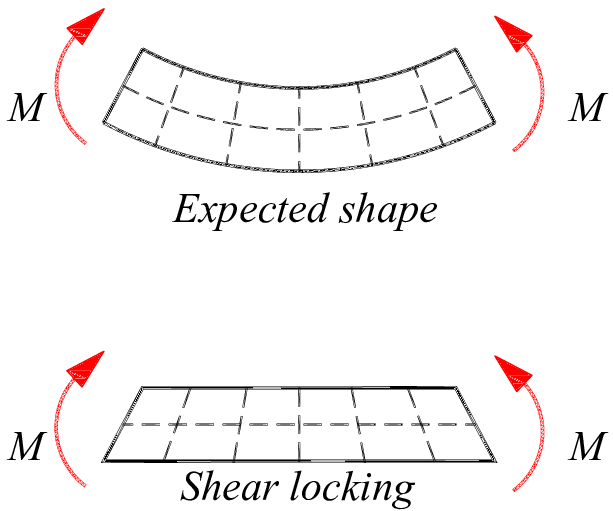
\includegraphics[width=3.5cm]{../images/shearLocking.png}
  \end{center}
  \begin{block}{}
    \begin{itemize}
      \item Reissner-Mindlin theory has demonstrated to suffer from \emph{shear locking}: as the thickness of the plate is reduced, the element becomes over-stiff and the computed displacements are much smaller than the analytical solution.
      \item The simplest remedy to this numerical behavior is to perform reduced integration of the shear component (\emph{selective integration}).
      \item For instance, if bilinear elements are used, then: \textbf{$2\times2$ Gauss integration (exact) for ${}^e\mathbf K_b$ and single point quadrature (reduced) for ${}^e\mathbf K_s$.}
    \end{itemize}
  \end{block}
\end{frame}

\begin{frame}{Elementary matrix and loads vector}
  \begin{block}{}
    \begin{itemize}
      \item \textbf{Elementary mass matrix} ($12\times 12$):
            $${}^e\mathbf M=\int_{{}^e\Omega}  {}^e\mathbf H^T\, \mathbf{I}\, {}^e\mathbf H \, d\Omega.$$
      \item \textbf{Elementary applied forces vector} ($12\times 1$):
            $${}^e\mathbf r(t)=\int_{{}^e\Omega} {}^e\mathbf H^{T}\mathbf f\, d\Omega.$$
    \end{itemize}
  \end{block}
\end{frame}

\begin{frame}{Post processing: stress recovery}
  Once the nodal generalized displacements ${}^e\mathbf{q}^i$ is computed out  stresses can be recovered from constitutive equations as:
  \begin{align*}
    \boldsymbol{\sigma}_b^h & = \mathbf C_b \boldsymbol{\varepsilon}_b^h = z \mathbf C_b\nabla_b {}^e\mathbf H {}^e\mathbf q = z \mathbf C_b{}^e \mathbf B_b{}^e\mathbf q, \\[5pt]
    \boldsymbol{\sigma}_s^h & =\mathbf C_s \boldsymbol{\varepsilon}_s^h = z \mathbf C_s\nabla_s {}^e\mathbf H {}^e\mathbf q = z \mathbf C_s{}^e \mathbf B_s{}^e\mathbf q.
  \end{align*}
  \vspace{-0.5cm}
  \begin{itemize}
    \item Bending stresses are linear through the plate thickness.
    \item  On the contrary, shear stresses are constant through the thickness, thus they are independent on $z$.
  \end{itemize}
\end{frame}

\section{Example: modal analysis of a simply supported thick plate}

\begin{frame}{Example: Simply supported square isotropic plate}
  \begin{enumerate}
    \item Approximate the first natural frequency of a  ($1\times1\times0.1$) plate, which is simply supported on all four edges.
          \vspace{0.3cm}
          \begin{center}
            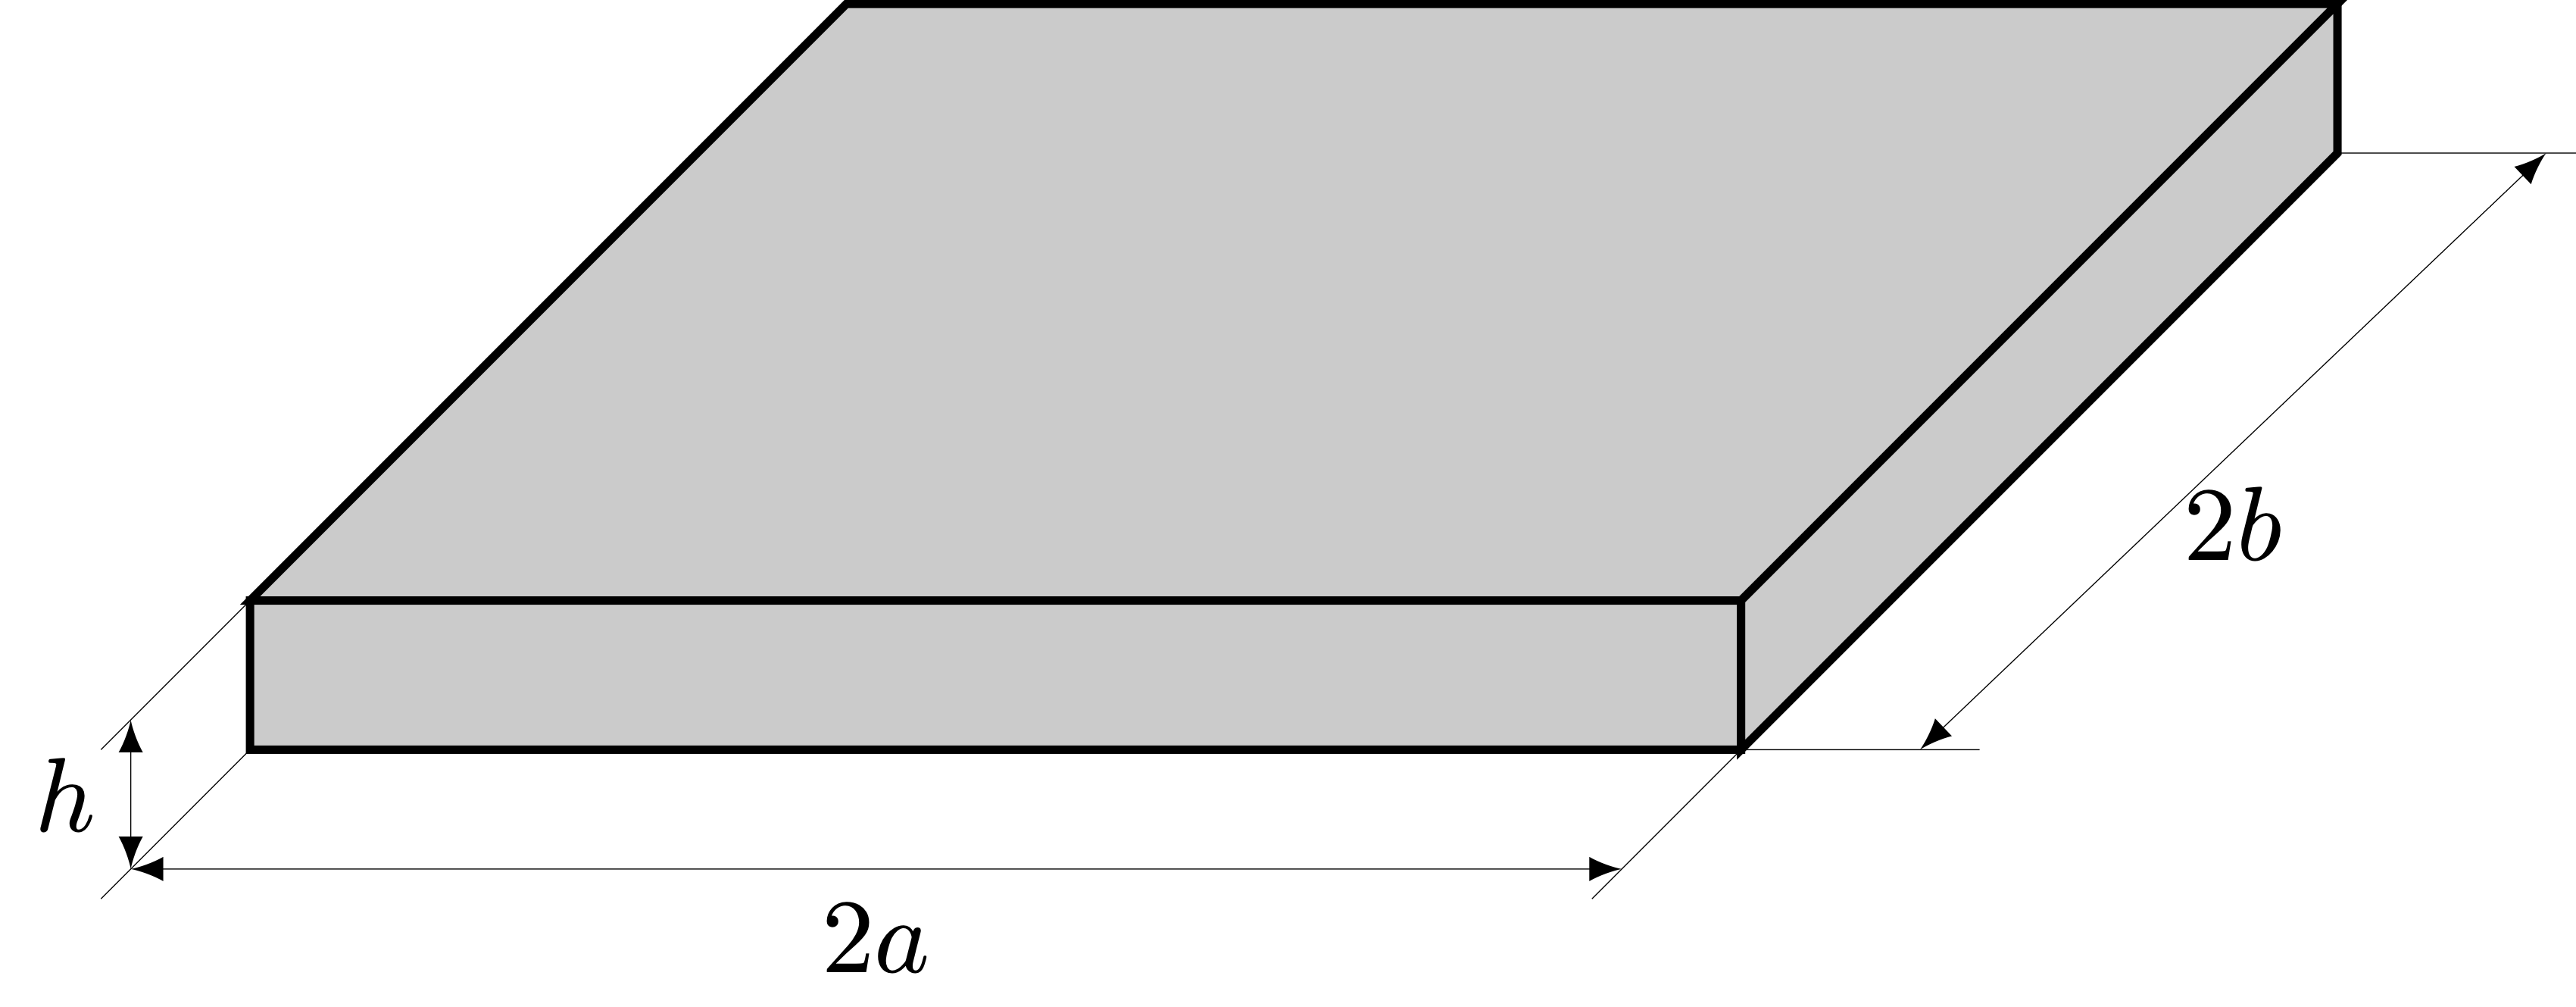
\includegraphics[width=5.5cm]{../images/plateModThick.png}
          \end{center}
    \item Compare the results with the analytical solution (as a function of $h$): $$\omega_{1,1}^{\text{exact}}(h) =10\pi h\sqrt{\frac{70}{4\pi^2h^2+7}}\ \text{Hz}.$$  Notice that this formula is only valid for the following choice of the plate geometry and materials.
  \end{enumerate}
\end{frame}

\begin{frame}{  Discretization with $4$ HTK elements}
  \begin{columns}
    \column{0.45\textwidth}
    \vspace{-0.5cm}
    \begin{center}
      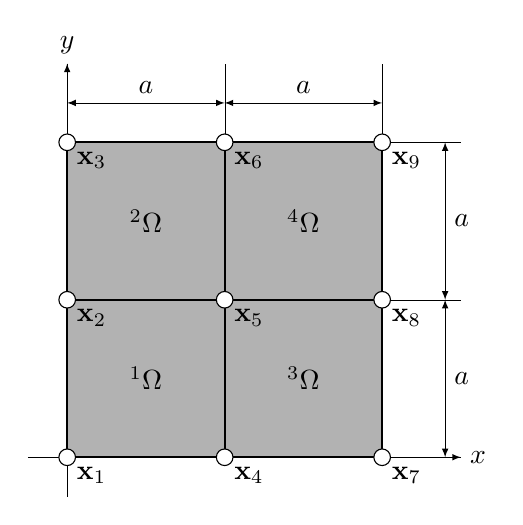
\begin{tikzpicture}[scale=1]
        \def\a{4}
        \def\b{4}
        % Draw the rectangle
        \filldraw[fill=gray!60, draw=black,thick] (0,0) rectangle (\a,\b);
        % Draw the elements  
        \draw[thick] (\a/2,0) -- (\a/2,\b);
        \draw[thick] (0,\b/2) -- (\a,\b/2);
        \node at (\a/4,\b/4) {${}^1\Omega$};
        \node at (\a/4,3*\b/4) {${}^2\Omega$};
        \node at (3*\a/4,\b/4) {${}^3\Omega$};
        \node at (3*\a/4,3*\b/4) {${}^4\Omega$};
        %axis
        \draw[-latex,ultra thin] (-0.5,0) -- (\a+1,0) node[right]{$x$};
        \draw[-latex, ultra thin] (0,-0.5) -- (0,\b+1)node[above]{$y$};
        % length
        \draw[latex-latex, ultra thin]  (0,\b+0.5)  to node[midway,above] {$a$}(\a/2,\b+0.5) ;
        \draw[latex-latex, ultra thin]  (\a/2,\b+0.5)  to node[midway,above] {$a$}(\a,\b+0.5) ;
        \draw[ultra thin] (\a/2,0) --(\a/2, \b+1);
        \draw[ultra thin] (\a,0) --(\a, \b+1) ;
        \draw[ultra thin] (0,\b/2) --(\a+1, \b/2);
        \draw[ultra thin] (0,\b) --(\a+1, \b);
        \draw[ultra thin] (\a,0) -- (\a+1,0);
        \draw[ultra thin] (0,\b) -- (0,\b+1);
        \draw[latex-latex, ultra thin]  (\a+0.8,\b/2)  to node[midway,right] {$a$}(\a+0.8,0) ;
        \draw[latex-latex, ultra thin]  (\a+0.8,\b)  to node[midway,right] {$a$}(\a+0.8,\b/2) ;
        % Nodes 
        \draw[fill=white, draw=black]  (0,0) node[below right]{$\mathbf x_1$} circle (3pt);
        \draw[fill=white, draw=black]  (0,\b/2) node[below right]{$\mathbf x_2$} circle (3pt);
        \draw[fill=white, draw=black]  (0,\b) node[below right]{$\mathbf x_3$} circle (3pt);
        \draw[fill=white, draw=black]  (\a/2,0) node[below right]{$\mathbf x_4$} circle (3pt);
        \draw[fill=white, draw=black]  (\a/2,\b/2) node[below right]{$\mathbf x_5$} circle (3pt);
        \draw[fill=white, draw=black]  (\a/2,\b) node[below right]{$\mathbf x_6$} circle (3pt);
        \draw[fill=white, draw=black]  (\a,0) node[below right]{$\mathbf x_7$} circle (3pt);
        \draw[fill=white, draw=black]  (\a,\b/2) node[below right]{$\mathbf x_8$} circle (3pt);
        \draw[fill=white, draw=black]  (\a,\b) node[below right]{$\mathbf x_9$} circle (3pt);
      \end{tikzpicture}
    \end{center}

    \column{0.6\textwidth}
    {\begin{itemize}\setlength\itemsep{0.05em}
        \item $2a=1$ length
        \item $2a=1$ height
        \item $h=0.1$ thickness
        \item $E=10920$ Young's modulus
        \item $\nu=0.3$ Poisson's ratio
        \item $\rho=1$ material density
        \item $k=5/6$ shear correction coefficient
      \end{itemize}}
    \vspace{0.2cm}
    The values for $\rho$ and $E$ is only a practical convenience to obtain non-dimensional flexural rigidity of the plate:
    $$D = \frac{E h^3}{12(1-\nu^2)}=1.$$
  \end{columns}
\end{frame}


\begin{frame}{Frequencies approximation for square plate with HTK elements}
  \vspace{-1cm}
  Comparison of exact and approximate natural frequencies with a mesh of $2\times 2$ HTK elements for a thick SSSS square plate.
  \vspace{0.3cm}
  \begin{table}[h!]
    \centering
    \begin{tabular}{ccccc}
      \hline
      $m$ & $n$ & Exact Freq. [Hz] & Approx. Freq. [Hz] & Rel. Error (\%) \\
      \hline
      1   & 1   & 9.6658           & 12.543             & 29.768          \\
      1   & 2   & 23.251           & 125.96             & 441.75          \\
      2   & 1   & 23.251           & 125.96             & 441.75          \\
      2   & 2   & 35.895           & 250.98             & 599.19          \\
      1   & 3   & 43.871           & 260.74             & 494.33          \\
      3   & 1   & 43.871           & 284.72             & 549             \\
      2   & 3   & 55.239           & 284.72             & 415.44          \\
      \hline
    \end{tabular}
  \end{table}
\end{frame}

\begin{frame}{Frequencies approximation for square plate with HTK elements}
  In these figures, we present the convergence and relative errors of the first five natural frequencies of a square plate, obtained using HTK elements for different mesh refinements.
  \vspace{-0.5cm}
  \begin{columns}
    \begin{column}{.48\textwidth}
      \begin{figure}[H]
        \begin{center}
          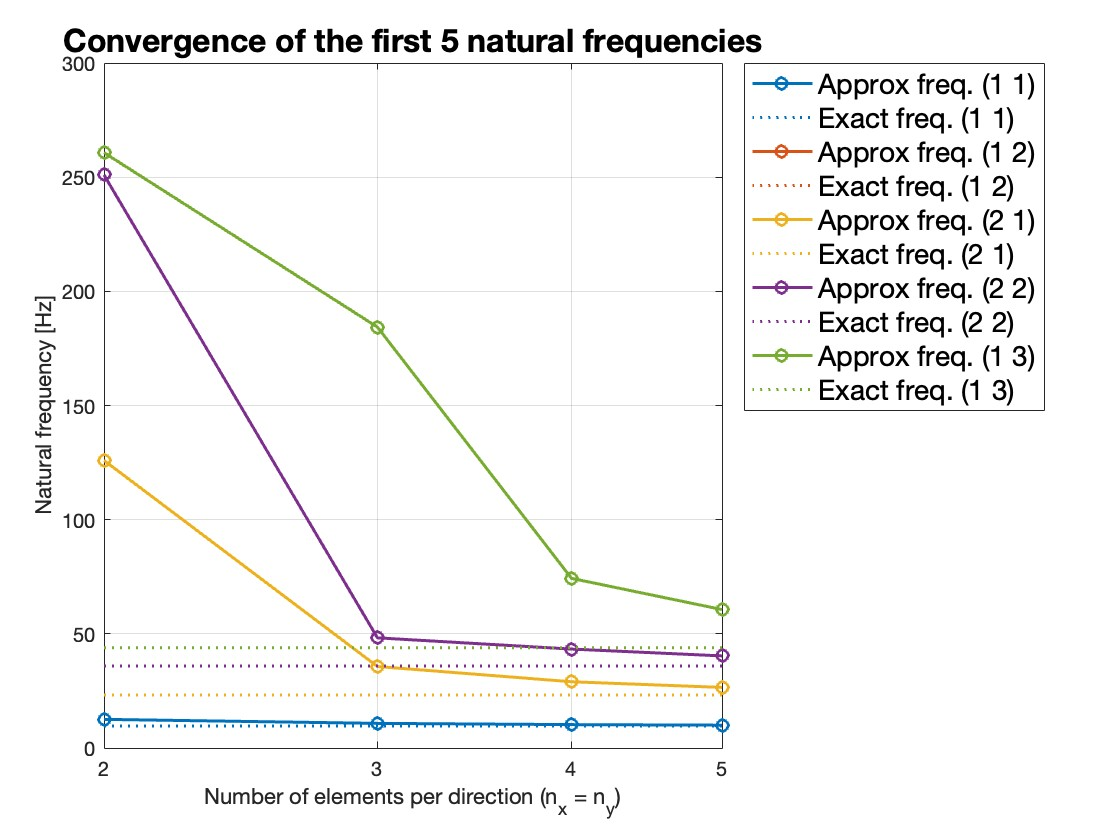
\includegraphics[height=5.5cm]{../images/HTKConv.jpg}
        \end{center}
      \end{figure}
    \end{column}
    \begin{column}{.48\textwidth}
      \begin{figure}[H]
        \begin{center}
          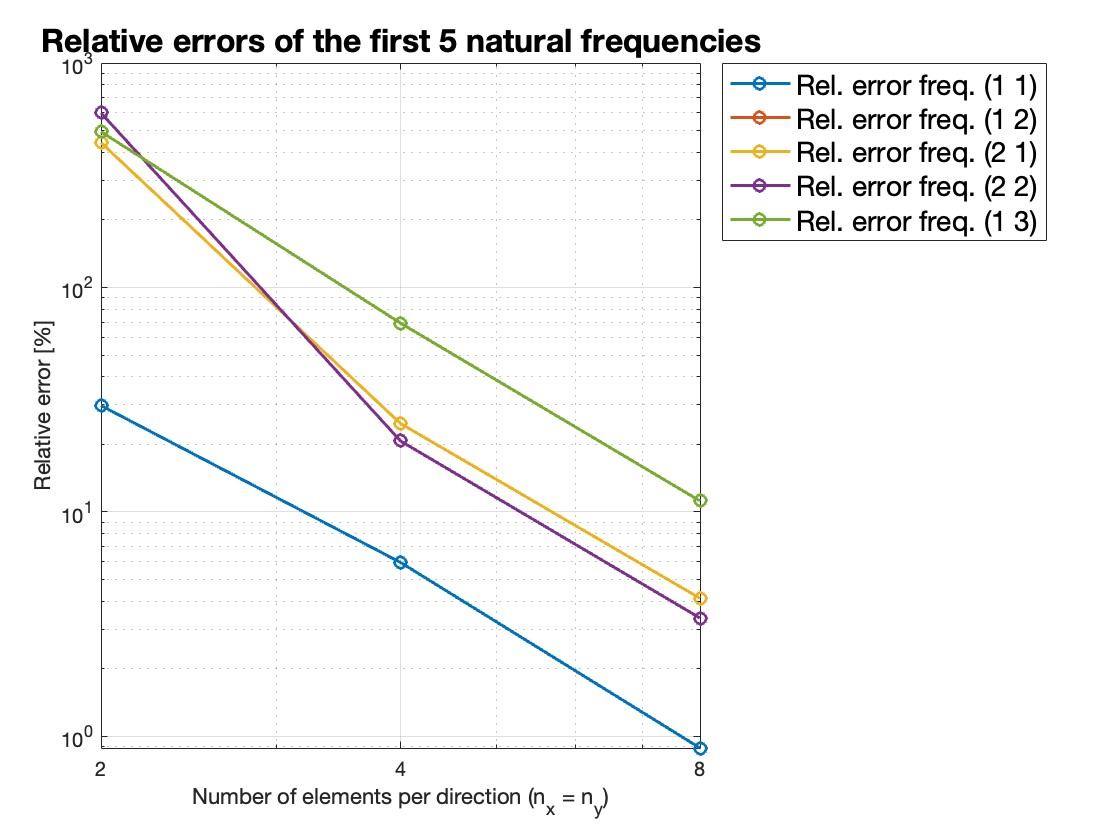
\includegraphics[height=5.5cm]{../images/HTKrelerr.jpg}
        \end{center}
      \end{figure}
    \end{column}
  \end{columns}
\end{frame}

\begin{frame}{Modal patterns}
  \begin{figure}[H]
    \begin{center}
      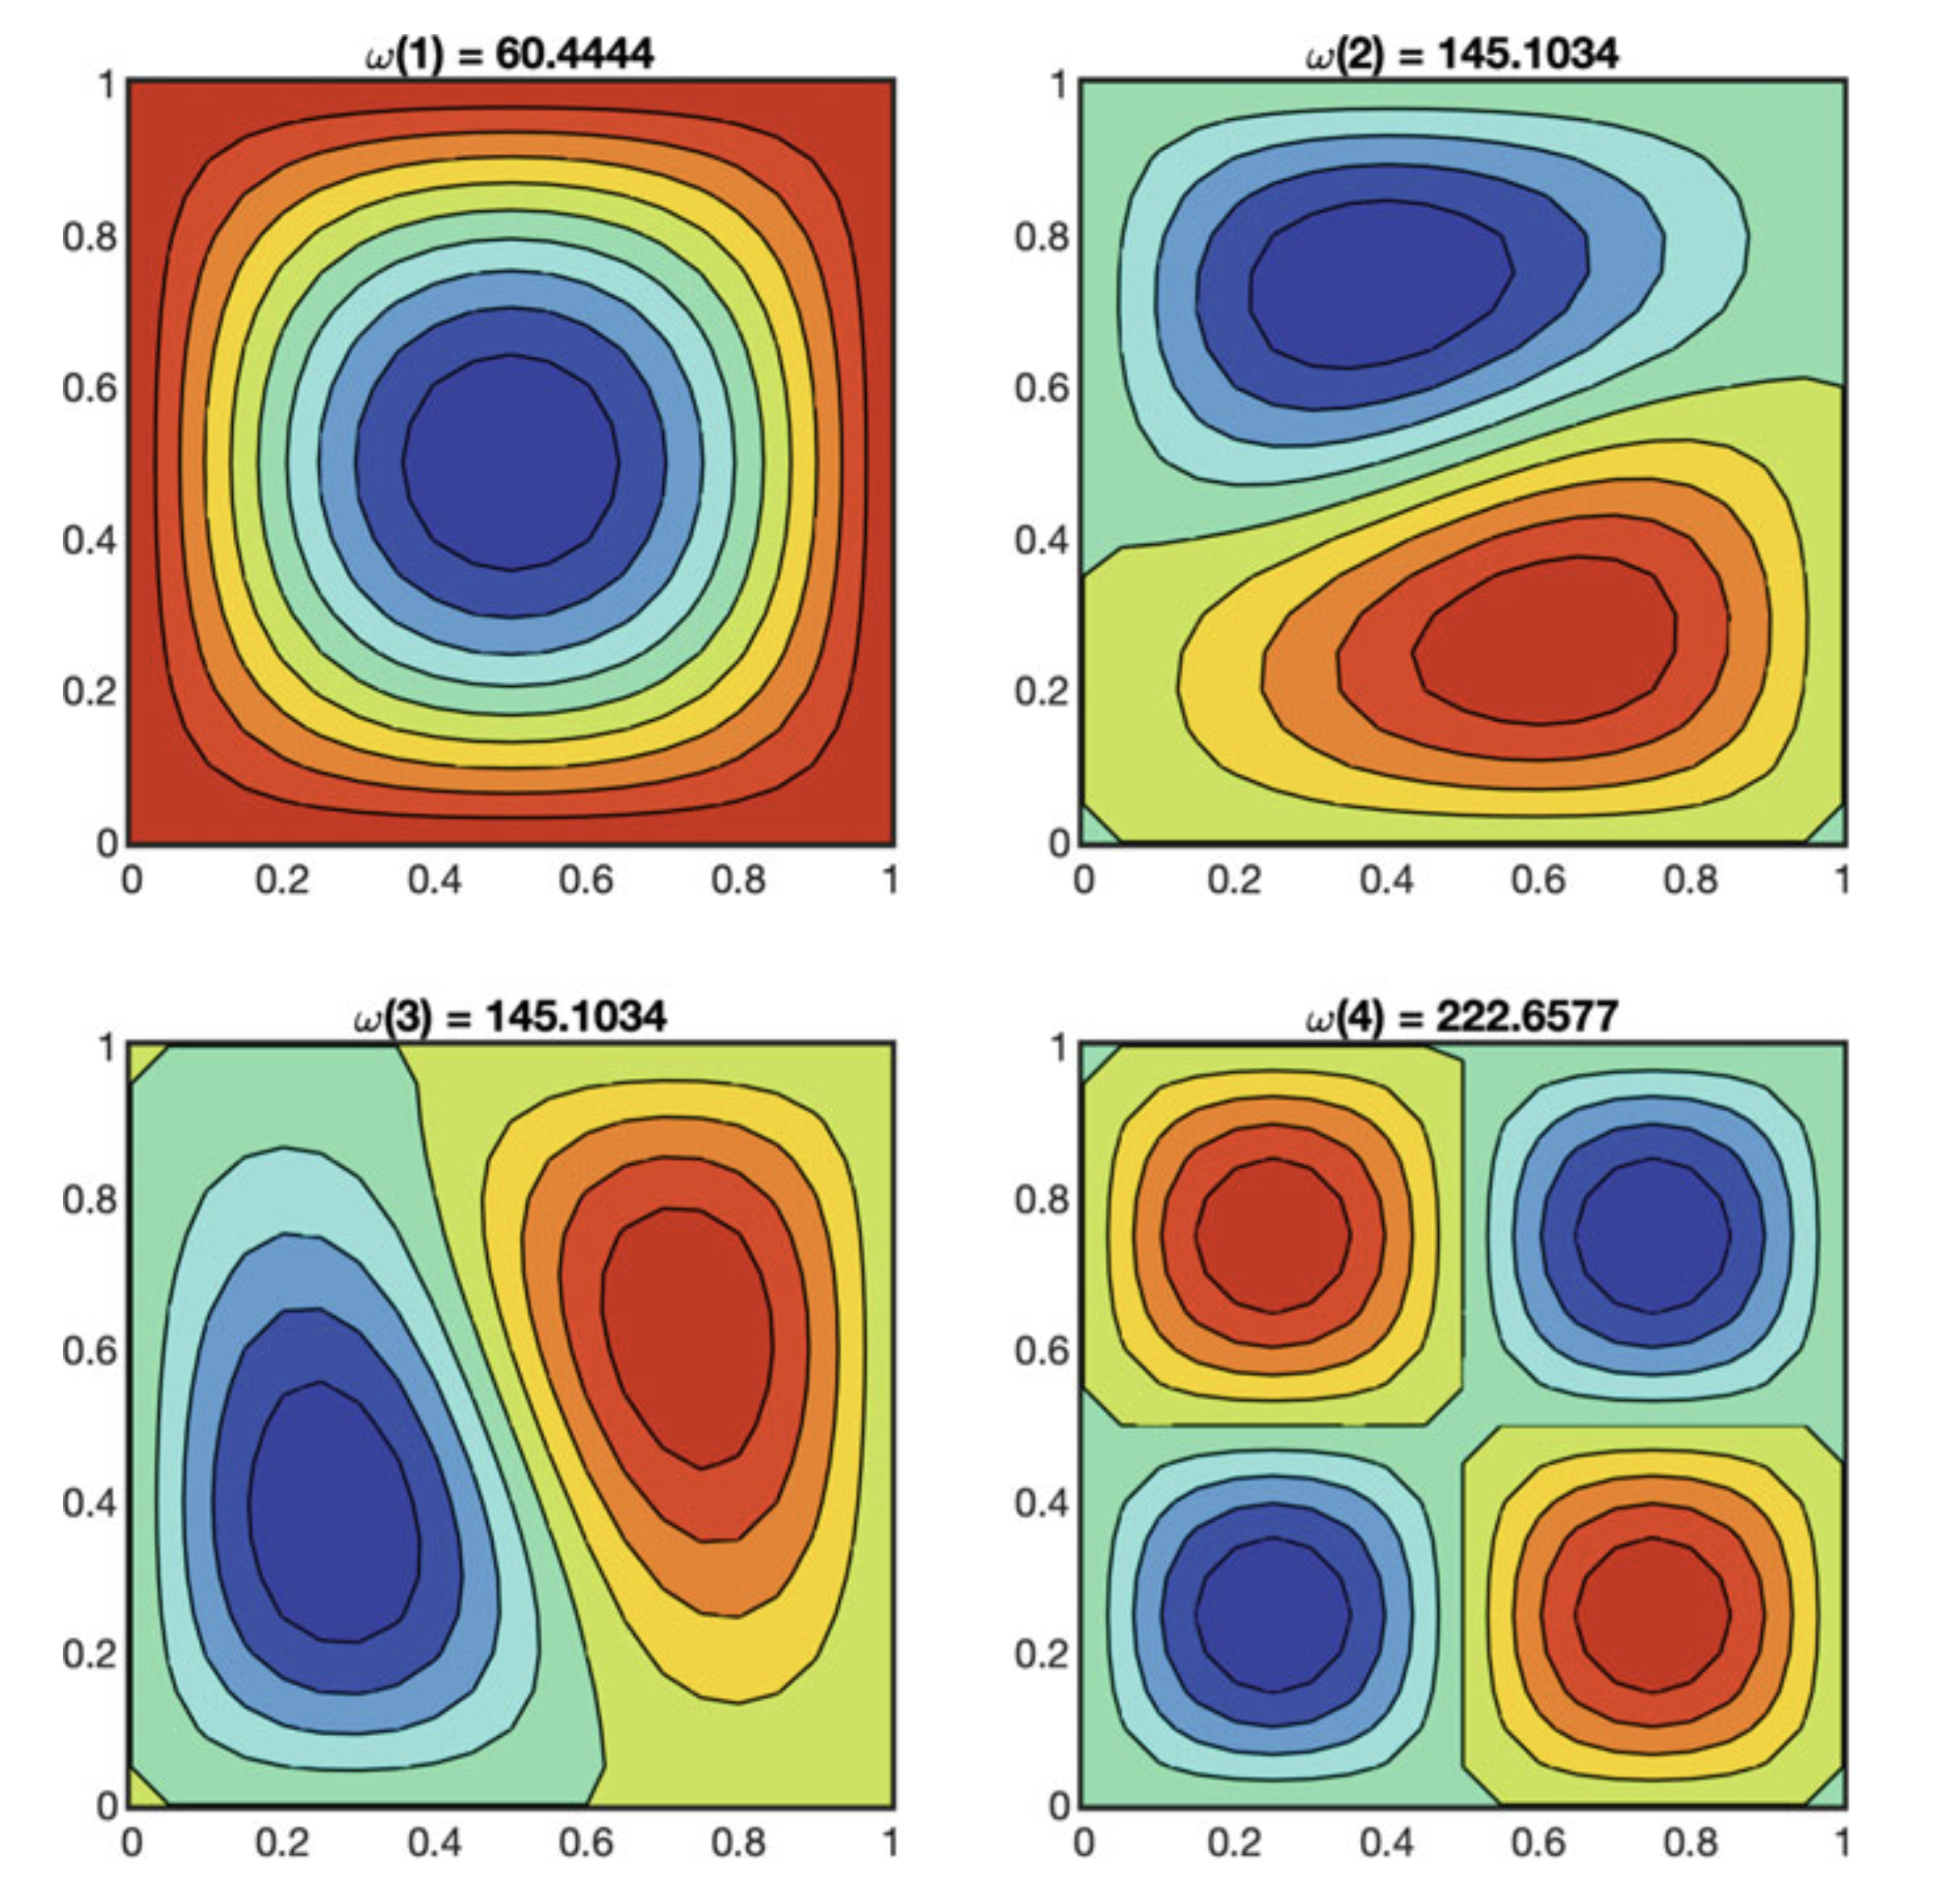
\includegraphics[height=5.5cm]{../images/modeShapeThickPlate.png}
      \caption{Modes of vibration for a SSSS plate with $h/a = 0.1$, using $20\times 20$ bilinear elements.}
    \end{center}
  \end{figure}
  \emph{\footnotesize (Credit: Ferreira, Fantuzzi - MATLAB Codes for Finite Element Analysis)}
\end{frame}

\end{document}